\documentclass[11pt,a4paper]{article}

\usepackage[utf8]{inputenc}
\usepackage[T1]{fontenc}
\usepackage{lmodern}
\usepackage[spanish,es-tabla]{babel}
\usepackage{amsmath,amssymb}
\usepackage{geometry}
\geometry{top=2.5cm, bottom=2.5cm, left=2.2cm, right=2.2cm}
\usepackage{circuitikz}
\usepackage{graphicx}
\usepackage{float}
\usepackage{booktabs}
\usepackage{xcolor}
\usepackage{microtype}
\usepackage{subcaption}
\usepackage{hyperref}

\hypersetup{
    colorlinks=true,
    linkcolor=blue!70!black,
    citecolor=blue!70!black,
    urlcolor=blue!70!black
}

\ctikzset{
    resistors/scale=0.65,
    capacitors/scale=0.65,
}

\title{\vspace{-1.2cm}
\includegraphics[height=2.5cm]{imagenes/logo_nandu_lsd.png}\\[0.6em]
\textbf{Informe Técnico: Optimización del Front-End sEMG con AD620}\\
\large Diagnóstico de Ruido de Línea, Mitigación de Despegue de Electrodos,\\
Arquitectura en Dos Etapas y Estrategia de Modificación Experimental}
\author{Proyecto Ñandú sEMG -- Laboratorio de Sistemas Dinámicos}
\date{Septiembre 2026}

\begin{document}

\maketitle

\begin{abstract}
En este informe se presenta el análisis técnico y diagnóstico del circuito de adquisición electromiográfica de superficie (sEMG) basado en el amplificador de instrumentación AD620. Se describe el origen de la hipersensibilidad al despegue de electrodos y la consecuente irrupción masiva de ruido de línea a 50~Hz debido a la colocación inadecuada de filtros $RC$ en las entradas diferenciales. Se formulan rigurosamente las ecuaciones bioeléctricas de interferencia de modo común y se desarrollan dos soluciones: una modificación inmediata sobre la placa actual mediante desacoplo de corriente alterna en el lazo de ganancia ($R_G + C_G$), y el rediseño formal recomendado bajo especificaciones SENIAM en dos etapas (AD620 a baja ganancia con filtro inter-etapa y amplificador secundario TL072 con filtrado anti-aliasing). Finalmente, se detalla una estrategia de modificación física no destructiva sobre el circuito impreso existente para validar la corrección de forma inmediata.
\end{abstract}

\tableofcontents
\newpage

% ====================================================================
\section{Diagnóstico del Circuito Actual y Mecanismos de Ruido}
% ====================================================================

El front-end analógico implementado originalmente consta de un amplificador de instrumentación AD620 alimentado por dos baterías de $\pm 9\,\text{V}$, con una resistencia de ganancia $R_G = 100\,\Omega$ y un filtro pasa-altos pasivo colocado inmediatamente en las entradas analógicas (capacitores serie de $33\,\text{nF}$ y resistencias a tierra de $100\,\text{k}\Omega$).

\begin{figure}[htbp]
\centering
\resizebox{0.88\textwidth}{!}{
\begin{circuitikz}[american, thick, font=\sffamily]

    % Título
    \node[font=\bfseries\large, anchor=west] at (-4.6, 3.4) {Circuito 1: Topología Original con Filtro RC a la Entrada - $R_G = 100\,\Omega$, $G \approx 495$};

    % AD620
    \draw[thick] (-1.0, 1.6) -- (2.0, 0) -- (-1.0, -1.6) -- cycle;
    \node at (0.4, 0) {\Large AD620};
    \node at (-0.65, 0.95) {\Large \(-\)};
    \node at (-0.65, -0.95) {\Large \(+\)};

    % Pines de Alimentación (±9V) y Referencia
    \draw[-latex] (-0.2, 1.17) -- ++(0, 0.9) node[above] {+9V};
    \node[left=1pt] at (-0.2, 1.35) {7};

    \draw[-latex] (-0.2, -1.17) -- ++(0, -0.9) node[below] {-9V};
    \node[left=1pt] at (-0.2, -1.35) {4};

    \draw (0.6, -0.75) -- ++(0, -0.9) node[ground]{};
    \node[right=2pt] at (0.6, -0.75) {5};

    \draw (2.0, 0) -- ++(1.4, 0) node[ocirc]{} node[pos=0.6, above] {6};

    % Pines 1 y 8 (Resistencia RG = 100 Ohm)
    \draw (-1.0, 0.45) node[right=3pt] {\scriptsize 1} -- (-2.0, 0.45) coordinate (r_top);
    \draw (-1.0, -0.45) node[right=3pt] {\scriptsize 8} -- (-2.0, -0.45) coordinate (r_bot);
    \draw (r_top) to[R, l_={\(100\,\Omega\)}, *-*] (r_bot);

    % Entradas con Filtro RC (33 nF + 100 k)
    \draw (-1.0, 1.05) node[left=2pt] {\scriptsize 2} -- (-3.2, 1.05) coordinate (juncA);
    \draw (juncA) to[R, l_={\(100\text{ k}\Omega\)}] ++(0, 1.5) node[ground, yscale=-1]{};
    \draw (juncA) to[C, l_={\(33\text{ nF}\)}] ++(-1.8, 0) node[left] {\(V_{\mathrm{in}}^-\)};

    \draw (-1.0, -1.05) node[left=2pt] {\scriptsize 3} -- (-3.2, -1.05) coordinate (juncB);
    \draw (juncB) to[R, l={\(100\text{ k}\Omega\)}] ++(0, -1.5) node[ground]{};
    \draw (juncB) to[C, l_={\(33\text{ nF}\)}] ++(-1.8, 0) node[left] {\(V_{\mathrm{in}}^+\)};

\end{circuitikz}
}
\caption{Circuito original. El filtro $RC$ a la entrada reduce la impedancia del canal a $100\,\text{k}\Omega$ y la asimetría de los capacitores degrada drásticamente el CMRR a 50~Hz.}
\label{fig:circuito_original}
\end{figure}

El sistema presenta los siguientes problemas críticos concatenados:

\subsection{Proximidad de la Frecuencia de Corte a la Frecuencia de Línea}
Con los componentes utilizados en la entrada ($R = 100\,\text{k}\Omega$ y $C = 33\,\text{nF}$), la frecuencia de corte teórica $f_c$ se calcula como:
\begin{equation}
f_c = \frac{1}{2\pi R C} = \frac{1}{2\pi \cdot (100 \times 10^3\,\Omega) \cdot (33 \times 10^{-9}\,\text{F})} \approx 48.23\,\text{Hz}
\end{equation}
Estar situado a solo $1.8\,\text{Hz}$ de la frecuencia de red ($50\,\text{Hz}$) es sumamente perjudicial:
\begin{itemize}
    \item Justo en la frecuencia de corte, la rotación de fase alcanza $+45^\circ$ y la pendiente de transferencia exhibe su máxima sensibilidad ante variaciones paramétricas.
    \item Los capacitores cerámicos comerciales poseen tolerancias de entre $\pm 10\%$ y $\pm 20\%$. Si una rama presenta $+10\%$ y la otra $-10\%$, una corta a $43.8\,\text{Hz}$ y la otra a $53.6\,\text{Hz}$.
    \item A $50\,\text{Hz}$, las entradas inversora y no inversora reciben señales atenuadas de forma dispar y fuertemente desfasadas en tiempo. Esta asimetría convierte la tensión en modo común ambiental en una tensión diferencial neta que el amplificador multiplica con una ganancia de $\approx 495$.
\end{itemize}

\subsection{Aplastamiento de la Impedancia de Entrada}
Aunque el AD620 posee una impedancia interna de entrada de $Z_{\text{chip}} \approx 10\,\text{G}\Omega$, la resistencia de polarización a tierra $R_{\text{ext}} = 100\,\text{k}\Omega$ queda conectada en paralelo hacia masa:
\begin{equation}
Z_{\text{in}} = R_{\text{ext}} \parallel Z_{\text{chip}} = \frac{100\,\text{k}\Omega \cdot 10\,\text{G}\Omega}{100\,\text{k}\Omega + 10\,\text{G}\Omega} \approx 100\,\text{k}\Omega
\end{equation}
La norma internacional SENIAM (\textit{Surface ElectroMyoGraphy for the Non-Invasive Assessment of Muscles}) exige taxativamente:
\begin{itemize}
    \item $Z_{\text{in}} > 100\,\text{M}\Omega$ para electrodos convencionales con gel conductor.
    \item $Z_{\text{in}} > 1000\,\text{M}\Omega$ ($1\,\text{G}\Omega$) para electrodos secos.
\end{itemize}
El circuito actual opera con una impedancia mil veces por debajo de la norma requerida para instrumentación biomédica.

\subsection{Mecanismo de Despegue del Electrodo}
Según la ecuación de conversión de modo común a diferencial formulada por Roberto Merletti y Philip Parker:
\begin{equation}
\frac{V_{\text{out}}}{A_d} \approx V_{\text{cm}} \left( \frac{\Delta Z}{Z_i} + \frac{A_c}{A_d} \right)
\end{equation}
donde $V_{\text{cm}}$ es la tensión de modo común de red acoplada al cuerpo, $Z_i$ es la impedancia de entrada, y $\Delta Z = |Z_1 - Z_2|$ es el desbalance de impedancia de contacto entre parches:
\begin{enumerate}
    \item \textbf{Con electrodo bien adherido:} La piel preparada con gel húmedo presenta $Z_1 \approx Z_2 \approx 5\text{--}10\,\text{k}\Omega$, con un desbalance residual típico de $\Delta Z \approx 1\,\text{k}\Omega$. Con $Z_i = 100\,\text{k}\Omega$, el factor de conversión es:
    \begin{equation}
    \frac{\Delta Z}{Z_i} = \frac{1\,\text{k}\Omega}{100\,\text{k}\Omega} = 0.01 \quad (1\%)
    \end{equation}
    Esto ya filtra varios milivoltios de ruido de $50\,\text{Hz}$.
    \item \textbf{Al despegarse o moverse un electrodo:} La pérdida de contacto o secado del gel incrementa la impedancia de ese polo a $50\,\text{k}\Omega$, $100\,\text{k}\Omega$ o valores del orden del megaohmio. El desbalance pasa a ser $\Delta Z \approx 50\text{--}100\,\text{k}\Omega$:
    \begin{equation}
    \frac{\Delta Z}{Z_i} \approx \frac{100\,\text{k}\Omega}{100\,\text{k}\Omega} = 1.0 \quad (100\%)
    \end{equation}
    Casi toda la tensión de modo común del sujeto se convierte en tensión diferencial directa. El AD620 toma ese voltio completo, lo multiplica por $495$ y satura la salida contra los rieles de batería ($\pm 9\,\text{V}$), o produce una oscilación masiva que enmascara las bioseñales faciales.
\end{enumerate}

\subsection{Atenuación de la Banda Muscular Útil}
La banda de energía fundamental para electromiografía facial abarca de $20\,\text{Hz}$ a $500\,\text{Hz}$. Al fijar la frecuencia de corte pasa-altos en $48.2\,\text{Hz}$, las componentes lentas del espectro (entre $20\,\text{Hz}$ y $45\,\text{Hz}$) sufren una atenuación de entre $-6\,\text{dB}$ y $-12\,\text{dB}$, perdiendo más del 60\% de su amplitud antes de alcanzar la etapa de amplificación.

% ====================================================================
\section{Propuesta 1: Modificación en una Etapa con Desacoplo de Alterna}
% ====================================================================

Para resolver estos problemas sobre la placa ya fabricada sin necesidad de manufacturar un circuito impreso nuevo, se implementa la técnica de desacoplo de corriente alterna en el lazo de ganancia (Merletti \& Parker, Sección 5.3.2, Fig. 5.6b).

\begin{figure}[htbp]
\centering
\resizebox{0.88\textwidth}{!}{
\begin{circuitikz}[american, thick, font=\sffamily]

    \node[font=\bfseries\large, anchor=west] at (-4.6, 3.4) {Circuito 2: Modificación en 1 Etapa - $R_G = 100\,\Omega$, $C_G = 100\,\mu\text{F}$, $G_{\text{AC}} \approx 495$};

    % AD620
    \draw[thick] (-1.0, 1.6) -- (2.0, 0) -- (-1.0, -1.6) -- cycle;
    \node at (0.4, 0) {\Large AD620};
    \node at (-0.65, 0.95) {\Large \(-\)};
    \node at (-0.65, -0.95) {\Large \(+\)};

    % Pines de Alimentación (±9V) y Referencia
    \draw[-latex] (-0.2, 1.17) -- ++(0, 0.9) node[above] {+9V};
    \node[left=1pt] at (-0.2, 1.35) {7};

    \draw[-latex] (-0.2, -1.17) -- ++(0, -0.9) node[below] {-9V};
    \node[left=1pt] at (-0.2, -1.35) {4};

    \draw (0.6, -0.75) -- ++(0, -0.9) node[ground]{};
    \node[right=2pt] at (0.6, -0.75) {5};

    \draw (2.0, 0) -- ++(1.4, 0) node[ocirc]{} node[pos=0.6, above] {6};

    % Lazo de ganancia horizontal (RG = 100 Ohm y CG = 100 uF para fc ≈ 16 Hz)
    \draw (-1.0, 0.45) node[right=3pt] {\scriptsize 1} 
          to[R, l_={\(100\,\Omega\)}, *-*] (-3.0, 0.45) coordinate (rg_left);
    \draw (-1.0, -0.45) node[right=3pt] {\scriptsize 8} 
          to[C, l={\(100\,\mu\text{F}\)}, *-*] (-3.0, -0.45) coordinate (cg_left);
    \draw (rg_left) -- (cg_left);

    % Entradas directas con alta impedancia (10M a GND)
    \draw (-1.0, 1.15) node[left=2pt] {\scriptsize 2} -- (-4.2, 1.15) coordinate (juncA);
    \draw (juncA) to[R, l_={\(10\text{ M}\Omega\)}] ++(0, 1.5) node[ground, yscale=-1]{};
    \draw (juncA) -- ++(-1.2, 0) node[left] {\(V_{\mathrm{in}}^-\)};

    \draw (-1.0, -1.15) node[left=2pt] {\scriptsize 3} -- (-4.2, -1.15) coordinate (juncB);
    \draw (juncB) to[R, l={\(10\text{ M}\Omega\)}] ++(0, -1.5) node[ground]{};
    \draw (juncB) -- ++(-1.2, 0) node[left] {\(V_{\mathrm{in}}^+\)};

\end{circuitikz}
}
\caption{Circuito modificado en 1 etapa. Se eliminan los capacitores de entrada, se sube la resistencia a tierra a $10\,\text{M}\Omega$ y se bloquea el offset DC mediante un capacitor $C_G$ en serie con $R_G$.}
\label{fig:circuito_modificado_1etapa}
\end{figure}

\subsection{Principio Físico y Matemático del Desacoplo en Pines 1 y 8}
Internamente, los pines 1 y 8 del AD620 se conectan a los emisores del par diferencial de entrada a través de dos resistencias de realimentación de $24.7\,\text{k}\Omega$ ($24.7\,\text{k}\Omega + 24.7\,\text{k}\Omega = 49.4\,\text{k}\Omega$). La ganancia diferencial para cualquier impedancia compleja $Z_G(s)$ conectada externamente es:
\begin{equation}
G(s) = 1 + \frac{49.4\,\text{k}\Omega}{Z_G(s)}
\end{equation}
Al colocar en serie una resistencia $R_G = 100\,\Omega$ y un capacitor bipolar $C_G = 100\,\mu\text{F}$, la impedancia neta en función de la frecuencia es:
\begin{equation}
Z_G(f) = R_G + \frac{1}{j 2\pi f C_G} \implies |Z_G(f)| = \sqrt{R_G^2 + \left( \frac{1}{2\pi f C_G} \right)^2}
\end{equation}
El comportamiento por bandas de frecuencia es:
\begin{itemize}
    \item \textbf{En Corriente Continua (\(f = 0\,\text{Hz}\)):} El capacitor se comporta como circuito abierto ($X_C \to \infty$), por lo que $|Z_G| \to \infty$. La ganancia estática resulta:
    \begin{equation}
    G_{\text{DC}} = 1 + \frac{49.4\,\text{k}\Omega}{\infty} = 1
    \end{equation}
    El potencial galvánico de media celda generado por la piel ($\pm 50\text{ a } \pm 100\,\text{mV}$) solo se amplifica por $1$. En el pin 6 se obtienen únicamente $100\,\text{mV}$, imposibilitando la saturación contra las baterías de $\pm 9\,\text{V}$.
    \item \textbf{En Frecuencia de Corte (\(f_c \approx 15.9\,\text{Hz}\)):}
    \begin{equation}
    f_c = \frac{1}{2\pi R_G C_G} = \frac{1}{2\pi \cdot 100\,\Omega \cdot 100\,\mu\text{F}} \approx 15.91\,\text{Hz}
    \end{equation}
    A esta frecuencia, $X_C = 100\,\Omega$, $|Z_G| = 141.4\,\Omega$ y la ganancia alcanza $G \approx 350$ (atenuación clásica de $-3\,\text{dB}$).
    \item \textbf{En Banda Muscular Útil (\(f \ge 20\,\text{Hz}\)):} La reactancia capacitiva decae rápidamente: a $50\,\text{Hz}$ es de $31.8\,\Omega$, a $100\,\text{Hz}$ de $15.9\,\Omega$, y a $500\,\text{Hz}$ de solo $3.2\,\Omega$. La impedancia queda dominada por $R_G = 100\,\Omega$ y la ganancia se restituye a $G_{\text{AC}} \approx 495$, conservando más del 78\% de la energía a $20\,\text{Hz}$ y más del 98\% de $100\,\text{Hz}$ en adelante.
\end{itemize}

\subsection{Rol de las Resistencias de Polarización de Diez Megaohmios}
Al retirar los capacitores de entrada, la señal entra directa a los pines 2 y 3. Las resistencias a masa deben elevarse a $10\,\text{M}\Omega$:
\begin{enumerate}
    \item \textbf{Drenaje de la corriente de polarización (\(I_B\)):} Los transistores de entrada del AD620 precisan una corriente continua constante de $I_B \approx 2\,\text{nA}$ hacia masa para operar en régimen activo lineal. Si se dejara el circuito abierto (sin resistencia a GND), las capacidades parásitas acumularían carga hasta derivar la tensión a los rieles. Con $10\,\text{M}\Omega$, la caída es de solo:
    \begin{equation}
    V_{\text{offset}} = I_B \cdot R_{\text{ext}} = 2\,\text{nA} \cdot 10\,\text{M}\Omega = 20\,\text{mV}
    \end{equation}
    un valor completamente seguro.
    \item \textbf{Inmunidad ante el despegue:} Con $Z_{\text{in}} \approx 10\,\text{M}\Omega$, ante un despegue que produzca $\Delta Z = 100\,\text{k}\Omega$, la relación de conversión se reduce cien veces:
    \begin{equation}
    \frac{\Delta Z}{Z_{\text{in}}} = \frac{100\,\text{k}\Omega}{10\,\text{M}\Omega} = 0.01 \quad (1\%)
    \end{equation}
    El amplificador se vuelve prácticamente inmune a las variaciones mecánicas de contacto del parche.
\end{enumerate}

% ====================================================================
\section{Propuesta 2: Rediseño en Dos Etapas bajo Estándar SENIAM}
% ====================================================================

Para una versión definitiva del hardware, la recomendación oficial de Merletti y el consorcio SENIAM es la \textbf{arquitectura distribuida en dos etapas}.

\begin{figure}[htbp]
\centering
\resizebox{0.95\textwidth}{!}{
\begin{circuitikz}[american, thick, font=\sffamily]

    \node[font=\bfseries\large, anchor=west] at (-4.2, 3.8) {Circuito 3: Rediseño 2 Etapas - $G_1 \approx 10$, $G_2 \approx 48$, $G_{\mathrm{tot}} \approx 470\text{--}495$};

    % ETAPA 1: AD620 (Baja ganancia para soportar DC offset de electrodos)
    \draw[thick] (-1.0, 1.6) -- (2.0, 0) -- (-1.0, -1.6) -- cycle;
    \node at (0.35, 0) {\large AD620};
    \node at (-0.65, 0.95) {\Large \(-\)};
    \node at (-0.65, -0.95) {\Large \(+\)};

    % Pines de Alimentación (±9V) y Referencia
    \draw[-latex] (-0.2, 1.17) -- ++(0, 0.8) node[above] {+9V};
    \node[left=1pt] at (-0.2, 1.35) {\scriptsize 4};

    \draw[-latex] (-0.2, -1.17) -- ++(0, -0.8) node[below] {-9V};
    \node[left=1pt] at (-0.2, -1.35) {\scriptsize 7};

    \draw (0.6, -0.75) -- ++(0, -0.8) node[ground]{};
    \node[right=2pt] at (0.6, -0.75) {\scriptsize 5};

    % RG para baja ganancia (G1 = 1 + 49.4k/5.6k ≈ 9.8)
    \draw (-1.0, 0.45) node[right=3pt] {\scriptsize 1} -- (-1.9, 0.45) coordinate (r_top);
    \draw (-1.0, -0.45) node[right=3pt] {\scriptsize 8} -- (-1.9, -0.45) coordinate (r_bot);
    \draw (r_top) to[R, l_={\(5.6\text{ k}\Omega\)}, *-*] (r_bot);

    % Entradas directas
    \draw (-1.0, 1.05) node[left=2pt] {\scriptsize 2} -- (-2.8, 1.05) coordinate (juncA);
    \draw (juncA) to[R, l_={\(10\text{ M}\Omega\)}] ++(0, 1.4) node[ground, yscale=-1]{};
    \draw (juncA) -- ++(-1.0, 0) node[left] {\(V_{\mathrm{in}}^-\)};

    \draw (-1.0, -1.05) node[left=2pt] {\scriptsize 3} -- (-2.8, -1.05) coordinate (juncB);
    \draw (juncB) to[R, l={\(10\text{ M}\Omega\)}] ++(0, -1.4) node[ground]{};
    \draw (juncB) -- ++(-1.0, 0) node[left] {\(V_{\mathrm{in}}^+\)};

    % FILTRO PASA-ALTOS INTER-ETAPA (fc ≈ 15 Hz)
    \draw (2.0, 0) node[above right] {\scriptsize 6} 
          to[C, l={\(470\text{ nF}\)}] (4.0, 0) coordinate (hp_node);
    \draw (hp_node) to[R, l_={\(22\text{ k}\Omega\)}, *-] (4.0, -1.8) node[ground]{};

    % ETAPA 2: OPERACIONAL TL072 (G2 ≈ 48 + PASA-BAJOS anti-aliasing fc ≈ 500 Hz)
    \draw[thick] (6.6, 1.3) -- (8.8, 0) -- (6.6, -1.3) -- cycle;
    \node at (7.4, 0) {\small TL072};
    \node at (6.9, 0.6) {\large \(+\)};
    \node at (6.9, -0.6) {\large \(-\)};

    % Entrada no inversora (+)
    \draw (hp_node) -- (5.2, 0) |- (6.6, 0.6);

    % Entrada inversora (-) y resistencia a tierra
    \draw (6.6, -0.6) -- (5.6, -0.6) coordinate (inv_junc);
    \draw (inv_junc) to[R, l={\(1\text{ k}\Omega\)}, *-] (5.6, -1.8) node[ground]{};

    % Salida
    \draw (8.8, 0) -- (10.6, 0) coordinate (out_final) node[ocirc]{} node[above] {\(V_{\mathrm{out}}\)};

    % Lazo de realimentación ortogonal
    \draw (inv_junc) -- (5.2, -0.6) -- (5.2, 2.3) coordinate (fb_in);
    \draw (9.6, 0) node[circ]{} -- (9.6, 2.3) coordinate (fb_out);

    % Resistor superior (Rf = 47k -> G2 = 1 + 47k/1k = 48)
    \draw (fb_in) |- (5.8, 2.8) to[R, l={\(47\text{ k}\Omega\)}] (9.0, 2.8) -| (fb_out);
    % Capacitor inferior (Cf = 6.8nF -> fc ≈ 500 Hz)
    \draw (fb_in) |- (5.8, 1.8) to[C, l_={\(6.8\text{ nF}\)}] (9.0, 1.8) -| (fb_out);

\end{circuitikz}
}
\caption{Circuito recomendado en dos etapas. La primera etapa opera con baja ganancia ($G_1 \approx 9.8$) para prevenir saturación por offset. El filtro inter-etapa elimina la continua sobre una señal unipolar, y la segunda etapa aporta la ganancia restante ($G_2 = 48$) y el corte pasa-bajos anti-aliasing a $500\,\text{Hz}$.}
\label{fig:circuito_recomendado_2etapas}
\end{figure}

\subsection{Estructura y Dimensionamiento de Componentes}
\begin{enumerate}
    \item \textbf{Etapa 1: Front-End de Instrumentación (AD620)}
    \begin{itemize}
        \item Entradas directas con $R_{\text{ext}} = 10\,\text{M}\Omega$ a tierra (preserva el CMRR máximo sin componentes reactivos asimétricos).
        \item Resistencia de ganancia $R_{G1} = 5.6\,\text{k}\Omega$, que fija una ganancia moderada:
        \begin{equation}
        G_1 = 1 + \frac{49.4\,\text{k}\Omega}{5.6\,\text{k}\Omega} \approx 9.82
        \end{equation}
        Un potencial de offset galvánico severo de $100\,\text{mV}$ produce solo $V_{\text{out, DC}} = 9.82 \times 100\,\text{mV} \approx 0.98\,\text{V}$, operando con amplio margen dinámico dentro de los $\pm 9\,\text{V}$ de las baterías.
    \end{itemize}

    \item \textbf{Inter-Etapa: Filtro Pasa-Altos Unipolar}
    \begin{itemize}
        \item Compuesto por $C_{\text{inter}} = 470\,\text{nF}$ y $R_{\text{inter}} = 22\,\text{k}\Omega$.
        \item Frecuencia de corte:
        \begin{equation}
        f_{c, \text{PA}} = \frac{1}{2\pi \cdot 22\,\text{k}\Omega \cdot 470\,\text{nF}} \approx 15.39\,\text{Hz}
        \end{equation}
        \item \textbf{Ventaja fundamental:} Al aplicarse sobre la salida ya unificada (referenciada a tierra o \textit{single-ended}), la tolerancia del capacitor no degrada en absoluto el CMRR del sistema.
    \end{itemize}

    \item \textbf{Etapa 2: Ganancia Secundaria y Pasa-Bajos Anti-Aliasing (TL072)}
    \begin{itemize}
        \item Configuración no inversora con $R_1 = 1\,\text{k}\Omega$ y $R_f = 47\,\text{k}\Omega$:
        \begin{equation}
        G_2 = 1 + \frac{R_f}{R_1} = 1 + \frac{47\,\text{k}\Omega}{1\,\text{k}\Omega} = 48
        \end{equation}
        \item Ganancia total de la cadena de acondicionamiento de señales:
        \begin{equation}
        G_{\text{tot}} = G_1 \cdot G_2 = 9.82 \cdot 48 \approx 471.4 \quad (\approx 495)
        \end{equation}
        \item Filtro pasa-bajos activo con $C_f = 6.8\,\text{nF}$ en paralelo con $R_f$:
        \begin{equation}
        f_{c, \text{PB}} = \frac{1}{2\pi R_f C_f} = \frac{1}{2\pi \cdot 47\,\text{k}\Omega \cdot 6.8\,\text{nF}} \approx 498.1\,\text{Hz}
        \end{equation}
        Atenúa armónicos residuales, ruido de conmutación e interferencias electromagnéticas por encima de la banda sEMG antes de la digitalización con la tarjeta DAQ.
    \end{itemize}
\end{enumerate}

% ====================================================================
\section{Cuadro Comparativo de Topologías}
% ====================================================================

\begin{table}[htbp]
\centering
\small
\resizebox{\textwidth}{!}{
\begin{tabular}{@{}llll@{}}
\toprule
\textbf{Parámetro} & \textbf{1. Original} & \textbf{2. Modificado (1 Etapa)} & \textbf{3. Recomendado (2 Etapas)} \\ \midrule
Arquitectura & In-Amp único (G directa) & In-Amp con desacoplo AC en $R_G$ & In-Amp baja G + Op-Amp activo \\
Ganancia AC ($G_{\text{AC}}$) & $\approx 495$ ($R_G = 100\,\Omega$) & $\approx 495$ ($R_G = 100\,\Omega$) & $\approx 471\text{--}495$ ($G_1 \approx 10, G_2 = 48$) \\
Ganancia DC ($G_{\text{DC}}$) & $495$ (Saturación) & $1.0$ (Sin saturación) & $0$ (Bloqueado por filtro inter-etapa) \\
Impedancia $Z_{\text{in}}$ & $\approx 100\,\text{k}\Omega$ & $\ge 10\,\text{M}\Omega$ & $\ge 10\,\text{M}\Omega$ a $1\,\text{G}\Omega$ \\
Frecuencia Pasa-Altos & $48.2\,\text{Hz}$ (Pérdida en sEMG) & $15.9\,\text{Hz}$ (Preserva banda útil) & $15.4\,\text{Hz}$ (Preserva banda útil) \\
Frecuencia Pasa-Bajos & Limitada por AD620 & Limitada por AD620 & $498\,\text{Hz}$ (Anti-aliasing activo) \\
Sensibilidad al Despegue & Crítica ($\Delta Z / Z_{\text{in}} \approx 1$) & Mínima ($\Delta Z / Z_{\text{in}} \le 0.01$) & Nula ($\Delta Z / Z_{\text{in}} \le 0.01$) \\
Preservación de CMRR & Destruida por caps. entrada & Máxima (entradas directas) & Máxima (entradas directas) \\
Implementación & Ya construida & Modificación inmediata sin PCB nuevo & Requiere rediseño de PCB \\
Cumplimiento SENIAM & No conforme & Aceptable para laboratorio & Cumplimiento estricto total \\ \bottomrule
\end{tabular}
}
\caption{Comparativa técnica de las tres topologías analizadas.}
\label{tab:comparativa}
\end{table}

% ====================================================================
\section{Formulación Matemática Completa y Desglose de Parámetros}
% ====================================================================

A continuación se detallan las ecuaciones físicas y analíticas que sustentan el acondicionamiento de las bioseñales.

\subsection{Ecuación General de Ganancia en el AD620}
\begin{equation}
G = 1 + \frac{49.4\,\text{k}\Omega}{R_G}
\end{equation}
\begin{itemize}
    \item $G$: Factor de amplificación diferencial de tensión en régimen estático (adimensional).
    \item $49.4\,\text{k}\Omega$: Resistencia interna equivalente de realimentación del circuito integrado ($24.7\,\text{k}\Omega + 24.7\,\text{k}\Omega$).
    \item $R_G$: Resistencia colocada entre los terminales 1 y 8 ($\Omega$).
\end{itemize}

\subsection{Ecuación de Interferencia de Modo Común de Merletti}
\begin{equation}
\frac{V_{\text{out}}}{A_d} \approx V_{\text{cm}} \left( \frac{\Delta Z}{Z_i} + \frac{A_c}{A_d} \right)
\end{equation}
\begin{itemize}
    \item $V_{\text{out}}$: Tensión total de salida del amplificador ($\text{V}$).
    \item $A_d$: Ganancia diferencial del amplificador ($\text{V/V}$, adimensional).
    \item $A_c$: Ganancia en modo común del amplificador ($\text{V/V}$, adimensional).
    \item $A_c / A_d$: Factor de rechazo en modo común inverso ($\text{CMRR}^{-1}$).
    \item $V_{\text{cm}}$: Tensión parásita de $50\,\text{Hz}$ acoplada capacitivamente desde la instalación eléctrica al cuerpo ($\text{V}$).
    \item $\Delta Z$: Desbalance entre las impedancias de contacto de los electrodos ($\Omega$).
    \item $Z_i$: Impedancia de entrada en modo común del amplificador ($\Omega$).
\end{itemize}

\subsection{Frecuencia de Corte de Filtros RC Pasa-Altos Pasivos}
\begin{equation}
f_c = \frac{1}{2\pi R C}
\end{equation}
\begin{itemize}
    \item $f_c$: Frecuencia de corte a $-3\,\text{dB}$ ($\text{Hz}$).
    \item $R$: Resistencia del filtro ($\Omega$).
    \item $C$: Capacidad del capacitor del filtro ($\text{F}$).
\end{itemize}

\subsection{Respuesta en Frecuencia de la Red Serie de Ganancia}
\begin{equation}
Z_G(f) = \sqrt{R_G^2 + \left( \frac{1}{2\pi f C_G} \right)^2}
\end{equation}
\begin{equation}
G(f) = 1 + \frac{49.4\,\text{k}\Omega}{Z_G(f)} = 1 + \frac{49.4\,\text{k}\Omega}{\sqrt{R_G^2 + \left(\frac{1}{2\pi f C_G}\right)^2}}
\end{equation}
\begin{itemize}
    \item $Z_G(f)$: Módulo de la impedancia entre pines 1 y 8 a la frecuencia $f$ ($\Omega$).
    \item $R_G$: Resistencia serie de ganancia ($100\,\Omega$).
    \item $C_G$: Capacidad del capacitor serie de desacoplo ($100\,\mu\text{F}$).
    \item $f$: Frecuencia armónica de la componente bioeléctrica ($\text{Hz}$).
    \item $G(f)$: Ganancia diferencial efectiva en función de la frecuencia (adimensional).
\end{itemize}

\subsection{Offset por Corriente de Polarización de Entrada}
\begin{equation}
V_{\text{offset}, I_B} = I_B \cdot R_{\text{ext}}
\end{equation}
\begin{itemize}
    \item $V_{\text{offset}, I_B}$: Tensión continua espuria generada en el terminal de entrada ($\text{V}$).
    \item $I_B$: Corriente de polarización del AD620 ($I_B \approx 0.5\text{ a } 2.0\,\text{nA}$).
    \item $R_{\text{ext}}$: Resistencia externa a tierra ($10\,\text{M}\Omega$).
\end{itemize}

\subsection{Ganancia y Filtro Pasa-Bajos en Segunda Etapa}
\begin{equation}
G_{\text{tot}} = \left( 1 + \frac{49.4\,\text{k}\Omega}{R_{G1}} \right) \cdot \left( 1 + \frac{R_f}{R_1} \right)
\end{equation}
\begin{equation}
f_{c, \text{PB}} = \frac{1}{2\pi R_f C_f}
\end{equation}
\begin{itemize}
    \item $G_{\text{tot}}$: Ganancia diferencial compuesta total (adimensional).
    \item $R_{G1}$: Resistencia de ganancia en el AD620 ($5.6\,\text{k}\Omega$).
    \item $R_1$: Resistencia de la entrada inversora del TL072 a tierra ($1\,\text{k}\Omega$).
    \item $R_f$: Resistencia de realimentación del TL072 ($47\,\text{k}\Omega$).
    \item $C_f$: Capacitor de realimentación del TL072 ($6.8\,\text{nF}$).
    \item $f_{c, \text{PB}}$: Frecuencia de corte superior anti-aliasing ($\text{Hz}$).
\end{itemize}

\subsection{Ecuación General de Transferencia de Tensión de Entrada a Salida y Desbalance Dinámico}
La tensión total observable en la salida del amplificador ($V_{\text{out}}$) depende no solo del rechazo de modo común estático, sino de la transferencia analógica integral de cada rama de entrada considerando el acoplamiento bioeléctrico, el potencial galvánico y el divisor resistivo formado entre la impedancia de contacto piel-electrodo y la impedancia de entrada del instrumento.

Para cada electrodo de entrada ($j \in \{1, 2\}$), la tensión real presente en el nodo analógico del circuito integrado ($V_{\text{in}, j}$) resulta de la atenuación del divisor de tensión:
\begin{equation}
V_{\text{in}, j}(t) = \alpha_j(t) \cdot V_{\text{fuente}, j}(t) = \frac{Z_{i, j}}{Z_{e, j}(t) + Z_{i, j}} \cdot \left[ V_{\text{cm}}(t) \pm \frac{V_{\text{emg}}(t)}{2} + V_{\text{DC}, j}(t) \right]
\end{equation}

donde:
\begin{itemize}
    \item $V_{\text{in}, j}(t)$: Tensión instantánea que ingresa efectivamente a la entrada inversora o no inversora del chip ($\text{V}$).
    \item $\alpha_j(t)$: Factor de transferencia o atenuación del divisor de tensión de entrada para el canal $j$ (adimensional, $0 \le \alpha_j \le 1$).
    \item $Z_{e, j}(t)$: Impedancia de contacto de la interfaz piel-electrodo del canal $j$ ($\Omega$), dependiente de la adhesión mecánica, hidratación del gel y presión de contacto.
    \item $Z_{i, j}$: Impedancia de entrada a tierra de la rama correspondiente del amplificador ($\Omega$).
    \item $V_{\text{cm}}(t)$: Tensión parásita de modo común inducida en el cuerpo por el entorno electromagnético ($\text{V}$).
    \item $V_{\text{emg}}(t)$: Biopotencial de acción muscular diferencial genuino generado por la despolarización de las fibras musculares ($\text{V}$, típicamente $10\text{--}500\,\mu\text{V}$).
    \item $V_{\text{DC}, j}(t)$: Potencial galvánico continuo de media celda electroquímica en la interfaz metal-electrolito ($\text{V}$, típicamente $\pm 50\text{ a } \pm 300\,\text{mV}$).
\end{itemize}

La tensión total de salida del amplificador de instrumentación, considerando una ganancia diferencial $A_d$, una ganancia en modo común $A_c$ y una tensión de referencia $V_{\text{REF}}$, se modela formalmente como:
\begin{equation}
V_{\text{out}}(t) = A_d \left[ V_{\text{in}, 1}(t) - V_{\text{in}, 2}(t) \right] + A_c \left[ \frac{V_{\text{in}, 1}(t) + V_{\text{in}, 2}(t)}{2} \right] + V_{\text{REF}}
\end{equation}

Sustituyendo la ecuación del divisor de entrada y expandiendo algebraicamente, la tensión de salida se desglosa en cuatro componentes físicos fundamentales:
\begin{align}
V_{\text{out}}(t) \approx & \underbrace{A_d \cdot \bar{\alpha}(t) \cdot V_{\text{emg}}(t)}_{\text{Señal sEMG amplificada}} + \underbrace{A_d \cdot \Delta\alpha(t) \cdot V_{\text{cm}}(t)}_{\text{Ruido de red por desbalance}} \nonumber \\
& + \underbrace{A_d \left[ \alpha_1(t) V_{\text{DC}, 1} - \alpha_2(t) V_{\text{DC}, 2} \right]}_{\text{Salto y deriva de continua}} + \underbrace{A_c \bar{\alpha}(t) V_{\text{cm}}(t)}_{\text{Modo común residual}}
\end{align}

donde:
\begin{equation}
\bar{\alpha}(t) = \frac{\alpha_1(t) + \alpha_2(t)}{2} \approx \frac{Z_i}{\bar{Z}_e(t) + Z_i}
\end{equation}
\begin{equation}
\Delta\alpha(t) = \alpha_1(t) - \alpha_2(t) = \frac{Z_i \cdot \left[ Z_{e, 2}(t) - Z_{e, 1}(t) \right]}{\left[ Z_{e, 1}(t) + Z_i \right] \cdot \left[ Z_{e, 2}(t) + Z_i \right]} \approx \frac{\Delta Z_e(t)}{Z_i} \quad (\text{para } Z_i \gg Z_e)
\end{equation}

\subsubsection{Mecanismo de Inestabilidad Dinámica por Despegue de Electrodos}
Esta formulación matemática general revela las tres consecuencias simultáneas e inmediatas que se suscitan cuando un electrodo pierde contacto mecánico ($Z_{e, 1} \gg Z_{e, 2}$):
\begin{enumerate}
    \item \textbf{Explosión del Ruido de Línea de 50 Hz:} El factor $\Delta\alpha(t)$ salta de $\approx 0.001$ a valores cercanos a $0.5\text{--}1.0$. La tensión de red ambiental $V_{\text{cm}}(t)$ se multiplica directamente por la ganancia diferencial completa $A_d \approx 495$, saturando instantáneamente los rieles de batería ($\pm 9\,\text{V}$).
    \item \textbf{Pérdida de la Simetría y Distorsión de la Amplitud Muscular:} Al caer $\alpha_1(t)$ a valores inferiores a $0.5$, la señal muscular diferencial $V_{\text{emg}}(t)$ ya no se transfiere de manera balanceada. La contracción se atenúa artificialmente y se introduce una distorsión morfológica en la envolvente del pulso muscular.
    \item \textbf{Salto Abrupto de Continua y Transitorio de Saturación:} La diferencia de potenciales galvánicos $(\alpha_1 V_{\text{DC}, 1} - \alpha_2 V_{\text{DC}, 2})$ experimenta un escalón instantáneo de tensión que se multiplica por $A_d$, desplazando violentamente la línea de base hacia los extremos del rango dinámico hasta que los lazos de acoplo logran reestabilizarse.
\end{enumerate}
Al elevar la impedancia de entrada a $Z_i \ge 10\,\text{M}\Omega$ (o $> 100\,\text{M}\Omega$ como prescribe SENIAM), el denominador del factor $\Delta\alpha(t)$ se incrementa en varios órdenes de magnitud, garantizando que $\Delta\alpha(t) \approx 0$ e inmunizando al front-end frente a las variaciones dinámicas de la interfaz cutánea.

% ====================================================================
\section{Análisis de Fenómenos No Lineales y Justificación de la Modificación Frente al Filtrado Digital}
% ====================================================================

Una interrogante fundamental en el acondicionamiento de biopotenciales es si resulta estrictamente necesario modificar físicamente el circuito de la placa, dado que las interferencias de línea a $50\,\text{Hz}$ y sus armónicos ($100$, $150$, $250\,\text{Hz}$) pueden suprimirse mediante técnicas de procesamiento digital (como filtros Notch en cascada o canceladores adaptativos NLMS en cuadratura).

El análisis físico y circuital demuestra que el problema crítico ante el despegue de electrodos no radica en la componente periódica de $50\,\text{Hz}$, sino en fenómenos no lineales de banda ancha y distorsiones irreversibles que ningún algoritmo por software puede reconstruir una vez digitalizada la señal.

\subsection{Salto Galvánico de Continua y Transitorio de Saturación}
La interfaz metal-electrolito-piel constituye una celda electroquímica con un potencial continuo $V_{\text{DC}} \in [50, 300]\,\text{mV}$. Ante una gesticulación facial, vibración o despegue parcial del parche:
\begin{itemize}
    \item La doble capa electroquímica se deforma bruscamente, modulando el potencial galvánico en el tiempo: $\Delta V_{\text{DC}}(t)$.
    \item Este transitorio no es una oscilación de $50\,\text{Hz}$, sino un escalón aperiódico de frecuencia ultralenta ($0.1\text{ a } 15\,\text{Hz}$).
\end{itemize}

En la topología actual sin desacoplo, el AD620 aplica su ganancia nominal directamente en corriente continua ($G_{\text{DC}} \approx 495$):
\begin{equation}
V_{\text{salida, DC}}(t) = 495 \cdot \Delta V_{\text{DC}}(t)
\end{equation}
Un micro-despegue o tracción mecánica que altere el potencial en apenas $\Delta V_{\text{DC}} = 20\,\text{mV}$ intenta producir:
\begin{equation}
V_{\text{salida}} = 495 \times 0.02\,\text{V} = 9.9\,\text{V}
\end{equation}
Al estar el sistema alimentado por baterías de $\pm 9\,\text{V}$, el amplificador colisiona inmediatamente contra el límite físico de saturación (*rail clipping*):
\begin{itemize}
    \item La salida se congela en una meseta plana a $+8.5\,\text{V}$ o $-8.5\,\text{V}$.
    \item \textbf{Pérdida irrecuperable de información:} Durante el bloqueo por saturación, la derivada temporal se anula y la actividad muscular queda borrada. Ningún filtro digital (Notch, Butterworth o aprendizaje profundo) puede restituir una señal cuya amplitud fue recortada por saturación física del hardware.
\end{itemize}

Con la modificación propuesta (capacitor $C_G = 100\,\mu\text{F}$ en serie con $R_G$):
\begin{equation}
G_{\text{DC}} = 1 \implies V_{\text{salida, DC}} = 1 \times 20\,\text{mV} = 20\,\text{mV}
\end{equation}
La línea base se desplaza únicamente $20\,\text{mV}$, evitando la saturación, manteniendo al amplificador en su zona lineal y preservando la señal muscular sin interrupciones.

\subsection{Modulación Espuria de la Ganancia y Pérdida de Simetría Bioeléctrica}
La tensión muscular genuina $V_{\text{emg}}$ transferida al circuito integrado depende del divisor resistivo formado por la impedancia de contacto del electrodo $Z_e$ y la impedancia de entrada $Z_i$:
\begin{equation}
V_{\text{in}} = V_{\text{emg}} \cdot \left( \frac{Z_i}{Z_e + Z_i} \right)
\end{equation}

En la placa actual con $Z_i = 100\,\text{k}\Omega$:
\begin{itemize}
    \item Con electrodo bien adherido ($Z_e \approx 5\,\text{k}\Omega$):
    \begin{equation}
    \frac{100\,\text{k}\Omega}{5\,\text{k}\Omega + 100\,\text{k}\Omega} \approx 0.95 \quad (\text{se transfiere el } 95\% \text{ del potencial})
    \end{equation}
    \item Ante un despegue parcial o secado del gel ($Z_e \approx 100\,\text{k}\Omega$):
    \begin{equation}
    \frac{100\,\text{k}\Omega}{100\,\text{k}\Omega + 100\,\text{k}\Omega} = 0.50 \quad (\text{se transfiere únicamente el } 50\% \text{ del potencial})
    \end{equation}
\end{itemize}

Esta caída del $50\%$ en la amplitud se origina por un fenómeno mecánico y no por relajación fisiológica. En esquemas de procesamiento multicanal basados en el balance de activación entre músculos (como los ratios entre milohioideo, digástrico y orbicular, o la normalización por el Supremo Tricanal $M_{\text{supremo}}$), este falseamiento destruye la coherencia de las envolventes. El software no puede distinguir si la amplitud decreció por fonación submáximal o por despegue del sensor.

Con la elevación de la impedancia a $Z_i \ge 10\,\text{M}\Omega$:
\begin{equation}
\frac{10\,\text{M}\Omega}{100\,\text{k}\Omega + 10\,\text{M}\Omega} \approx 0.99 \quad (99\%)
\end{equation}
La amplitud bioeléctrica permanece invariable con un error inferior al $1\%$, independientemente de las fluctuaciones de contacto.

\subsection{Ruido Térmico de Johnson y Ruido de Corriente de Banda Ancha}
El despegue no solo introduce armónicos de red, sino ruido distribuido en todo el espectro sEMG ($20\text{ a }500\,\text{Hz}$):
\begin{enumerate}
    \item \textbf{Ruido Térmico en la Piel:}  
    \begin{equation}
    v_n = \sqrt{4 k_B T \cdot \text{Re}(Z_e) \cdot \Delta f}
    \end{equation}
    donde $k_B$ es la constante de Boltzmann ($1.38 \times 10^{-23}\,\text{J/K}$), $T$ es la temperatura absoluta en Kelvin ($310\,\text{K}$) y $\Delta f$ es el ancho de banda ($500\,\text{Hz}$). Al despegarse el electrodo, el área efectiva disminuye y $Z_e$ salta de $5\,\text{k}\Omega$ a $100\,\text{k}\Omega$, multiplicando por casi cinco veces el piso de ruido blanco térmico en toda la banda pasante.
    \item \textbf{Ruido de Corriente del Amplificador ($i_n$):}  
    El AD620 presenta una densidad de corriente de ruido de $i_n \approx 100\,\text{fA}/\sqrt{\text{Hz}}$. Al circular por una asimetría de contacto $\Delta Z_e$, genera una tensión de ruido diferencial:
    \begin{equation}
    v_{\text{ruido}} = i_n \cdot \Delta Z_e
    \end{equation}
    Este ruido es de naturaleza estocástica continua en el rango de $20\,\text{Hz}$ a $1\,\text{kHz}$, por lo que los filtros Notch centrados en $50\,\text{Hz}$ resultan totalmente ineficaces para eliminarlo.
\end{enumerate}

\subsection{Impacto del Filtro de Entrada en Cincuenta Hertz sobre la Bioseñal Facial}
Mantener el filtro pasa-altos $RC$ de entrada ($C = 33\,\text{nF}$, $R = 100\,\text{k}\Omega$) con frecuencia de corte en $f_c \approx 48.2\,\text{Hz}$ introduce fallas intrínsecas graves:
\begin{enumerate}
    \item \textbf{Atenuación Severa del Espectro sEMG Lento:}  
    La densidad espectral de potencia del electromiograma facial presenta componentes cardinales de reclutamiento motor entre $20\,\text{Hz}$ y $45\,\text{Hz}$. La curva de transferencia $|H(f)| = \frac{f/f_c}{\sqrt{1 + (f/f_c)^2}}$ arroja:
    \begin{itemize}
        \item A $20\,\text{Hz}$: $|H(20)| \approx 0.38$ (pérdida del $62\%$ de la amplitud).
        \item A $30\,\text{Hz}$: $|H(30)| \approx 0.53$ (pérdida del $47\%$ de la amplitud).
        \item A $40\,\text{Hz}$: $|H(40)| \approx 0.64$ (pérdida del $36\%$ de la amplitud).
    \end{itemize}
    El filtro analógico previo suprime más de la mitad de la información biomecánica antes de la digitalización.
    \item \textbf{Desfase Asimétrico y Generación de Tensión Diferencial:}  
    A $f_c$, la rotación de fase es de $+45^\circ$. Una disparidad de solo $\pm 10\%$ en la tolerancia entre capacitores desfasa una entrada respecto de la otra en $\Delta\phi \approx 8^\circ$. La diferencia vectorial convierte la tensión de modo común ambiental $V_{\text{cm}}$ en tensión diferencial:
    \begin{equation}
    V_{\text{diff}}(t) \approx 2 V_0 \sin\left(\frac{\Delta\phi}{2}\right) \cos(\omega t) \approx 0.14 \cdot V_0
    \end{equation}
    Para $V_0 = 1\,\text{V}$, se generan $140\,\text{mV}$ diferenciales que, multiplicados por $G=495$, dan $69.3\,\text{V}$, saturando los rieles.
    \item \textbf{Picos de Corriente Transitorios ($i = C \frac{dV}{dt}$):}  
    Ante un tirón mecánico del cable, la variación abrupta del potencial de contacto inyecta pulsos transitorios de corriente que despolarizan internamente el AD620 durante cientos de milisegundos.
    \item \textbf{Impedancia de Entrada Reactiva:}  
    A $50\,\text{Hz}$, la reactancia capacitiva es $X_C \approx 96.5\,\text{k}\Omega$. El módulo neto $|Z_{\text{in}}| = \sqrt{R^2 + X_C^2} \approx 139\,\text{k}\Omega$ introduce desfases variables dependientes de la impedancia cutánea, deformando la morfología del pulso.
\end{enumerate}

\subsection{Cuadro Comparativo entre Filtrado Digital y Modificación de Hardware}

\begin{table}[htbp]
\centering
\small
\resizebox{\textwidth}{!}{
\begin{tabular}{@{}lll@{}}
\toprule
\textbf{Fenómeno ante Despegue / Movimiento} & \textbf{Eficacia del Filtrado Digital (Notch / ANC)} & \textbf{Eficacia de la Modificación en Hardware ($R_G+C_G$, $10\,\text{M}\Omega$)} \\ \midrule
Ruido de línea a 50 Hz & Alta (elimina componentes senoidales) & Alta (elimina la conversión modo común a diferencial) \\
Saturación contra rieles ($\pm 9\,\text{V}$) & Nula (información destruida por clipping) & Total (fija $G_{\text{DC}}=1$, evitando saturación) \\
Caída de amplitud del 50\% en contracción & Nula (el software no distingue despegue de relajación) & Total (mantiene $Z_{\text{in}} \ge 10\,\text{M}\Omega$, transferencia al 99\%) \\
Ruido térmico blanco (20–500 Hz) & Nula (el Notch solo afecta 50 Hz) & Alta (reduce la inyección de corriente de ruido) \\
Atenuación muscular lenta (20–45 Hz) & Nula (energía ya eliminada por el filtro analógico) & Total (desplaza el corte a 15.9 Hz, recuperando la banda) \\ \bottomrule
\end{tabular}
}
\caption{Comparativa de alcances entre la corrección por software y el acondicionamiento analógico modificado.}
\label{tab:comparativa_software_hardware}
\end{table}

% ====================================================================
\section{Estrategia Experimental: Modificación en Placa sin Desoldar}
% ====================================================================

Para validar la modificación de 1 etapa de forma ágil, segura y 100\% reversible sin desmontar el PCB ni arriesgar pistas:

\subsection{Paso 1: Puentear los Capacitores de Entrada desde Arriba}
\begin{itemize}
    \item Tomar dos trozos de alambre de cobre fino pelado.
    \item Enrollar firmemente un alambre uniendo las dos patas expuestas de cada uno de los capacitores cerámicos de $33\,\text{nF}$ ubicados junto a las entradas 2 y 3.
    \item \textbf{Verificación con multímetro:} Medir continuidad entre el pad de entrada y los pines 2 y 3; debe registrar $0\,\Omega$.
\end{itemize}

\subsection{Paso 2: Inserción del Capacitor en el Lazo de Ganancia}
En la placa física, la resistencia azul de ganancia ($R_G = 100\,\Omega$) se encuentra elevada varios milímetros por encima del zócalo del integrado:
\begin{itemize}
    \item Con un alicate de corte al ras pequeño, cortar por la mitad una sola de las patas largas de $R_G$.
    \item Quedan dos terminales de alambre rígido expuestos mirando hacia arriba.
    \item Soldar o amarrar los terminales de un capacitor no polarizado de $100\,\mu\text{F}$ (o dos electrolíticos de $220\,\mu\text{F}$ en antiserie) entre los dos extremos cortados.
    \item \textbf{Ventaja:} No se toca el chip AD620, no se doblan patas y la red queda conectada en serie ($R_G + C_G$).
\end{itemize}

\subsection{Paso 3: Validación Inicial con Resistencias de Cien Kilo-ohmios}
Para la primera prueba de funcionamiento, \textbf{no es necesario desoldar las resistencias de \(100\,\text{k}\Omega\)}:
\begin{itemize}
    \item Las resistencias de $100\,\text{k}\Omega$ actuales drenan eficazmente la corriente $I_B$.
    \item Como el capacitor $C_G$ fija $G_{\text{DC}} = 1$, la salida no saturará contra los $\pm 9\,\text{V}$.
    \item Encender la placa y verificar que la línea base oscile libremente cerca de $0\,\text{V}$ sin topar los rieles.
\end{itemize}

\subsection{Paso 4: Elevación a Diez Megaohmios para Blindaje Frente a Despegue}
Una vez comprobado que la señal muscular entra limpia:
\begin{itemize}
    \item Cortar una sola pata de cada una de las resistencias de $100\,\text{k}\Omega$ a GND.
    \item Empalmar en su lugar resistencias de $10\,\text{M}\Omega$ (o mínimo $4.7\,\text{M}\Omega$) para elevar $Z_{\text{in}}$ a más de $10\,\text{M}\Omega$.
\end{itemize}

\subsection{Paso 5: Fijación Mecánica de Cables y Referencia en Mastoides}
\begin{itemize}
    \item El despegue se origina por la tracción del peso del cable sobre el electrodo facial. Asegurar el cable con cinta médica adhesiva sobre el cuello o la mandíbula, dejando los últimos $5\text{--}8\,\text{cm}$ holgados hacia el parche.
    \item Limpiar exhaustivamente con alcohol la apófisis mastoides para que el electrodo de referencia drene con baja impedancia el potencial de modo común corporal.
\end{itemize}

% ====================================================================
\section{Evidencia Bibliográfica del Tratado de Merletti y Parker}
% ====================================================================

A continuación se adjuntan las páginas pertinentes del libro oficial \textit{Electromyography: Physiology, Engineering, and Noninvasive Applications} (Roberto Merletti y Philip A. Parker, IEEE Press / John Wiley \& Sons, 2004), extraídas directamente del tratado de referencia.

\subsection{Requisitos de Entrada y Rechazo de Modo Común}
La página 115 formaliza los requerimientos de la instrumentación de entrada: ultra-alta impedancia para evitar carga galvánica, bajo ruido referido a la entrada y alto CMRR para rechazar la interferencia ambiental de red.

\begin{figure}[htbp]
\centering
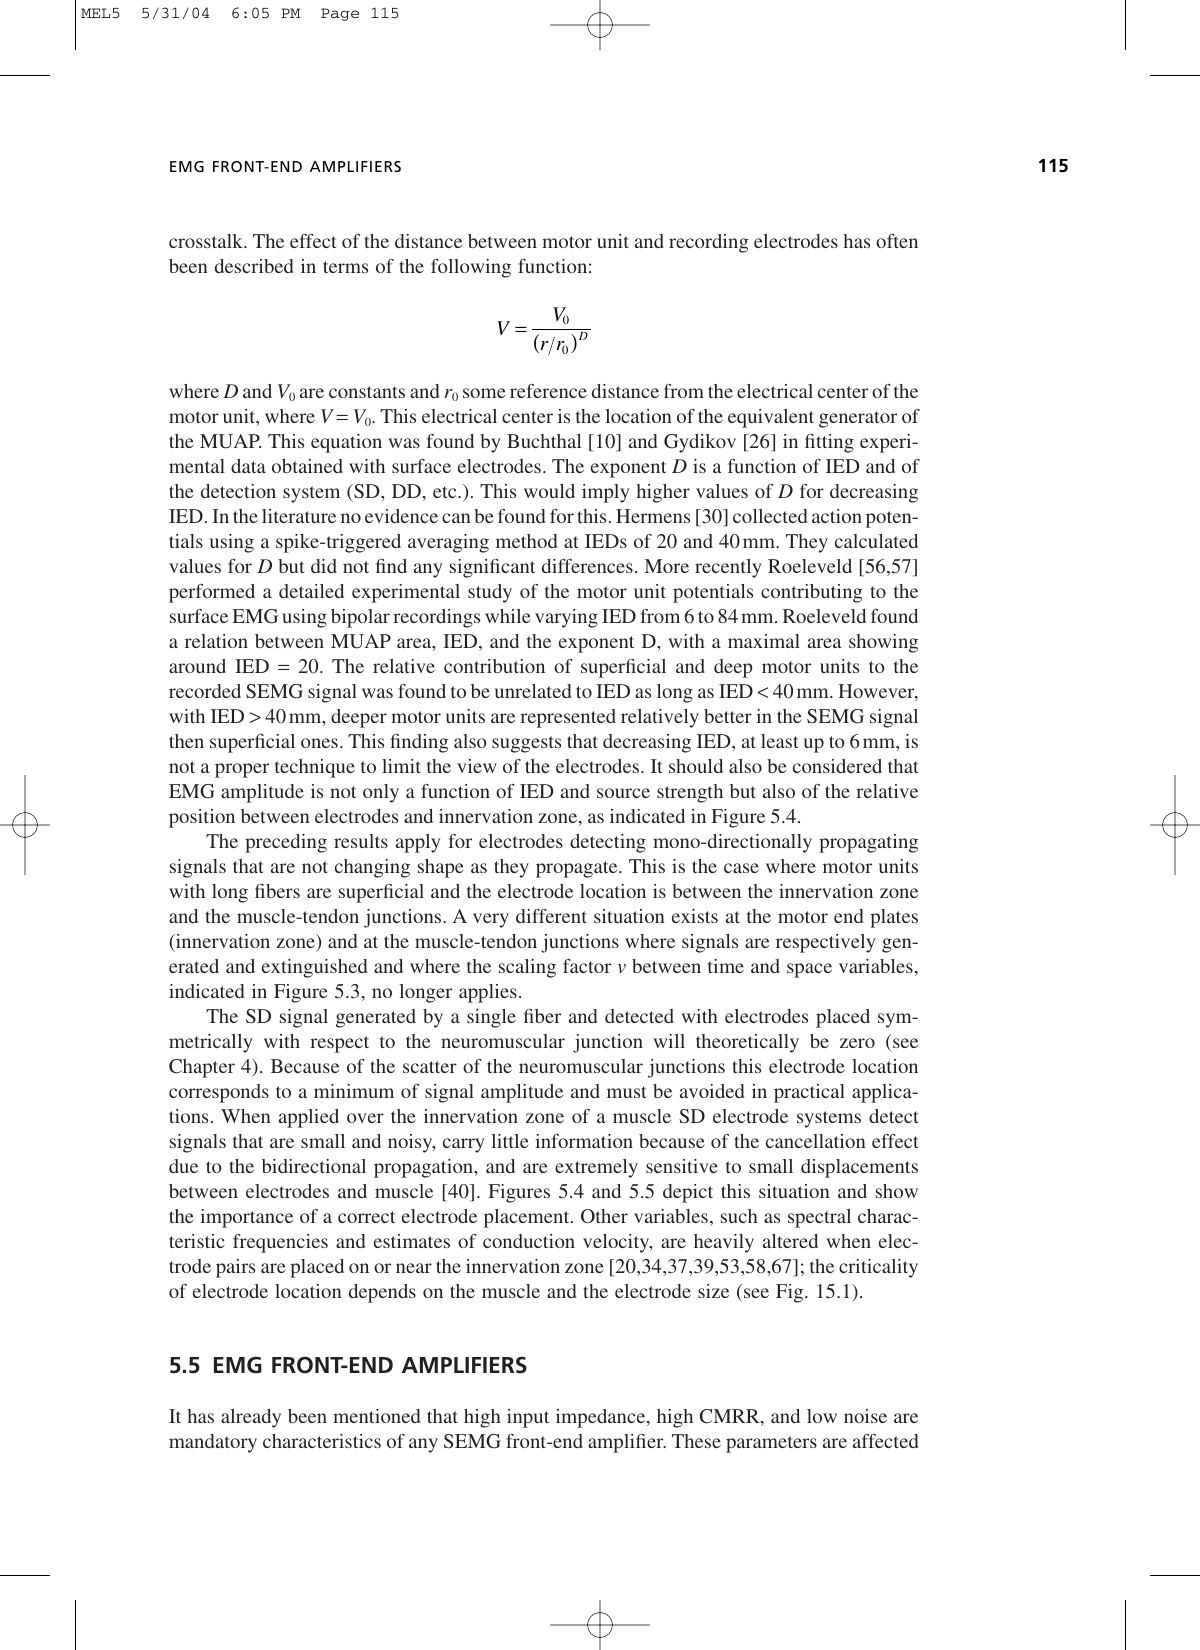
\includegraphics[width=0.82\textwidth]{imagenes/captura_merletti_sec5_5-136.png}
\caption{Página 115 del tratado de Merletti y Parker (2004). Introducción a los requisitos fundamentales de los amplificadores de entrada para sEMG.}
\label{fig:merletti_p115}
\end{figure}

\subsection{Justificación de la Impedancia Superior a Cien Megaohmios}
La página 116 establece que la impedancia de entrada debe superar en al menos dos órdenes de magnitud la impedancia de la piel con gel ($> 100\,\text{M}\Omega$) y superar $1000\,\text{M}\Omega$ ($1\,\text{G}\Omega$) para electrodos secos, explicando el efecto del divisor capacitivo de entrada.

\begin{figure}[htbp]
\centering
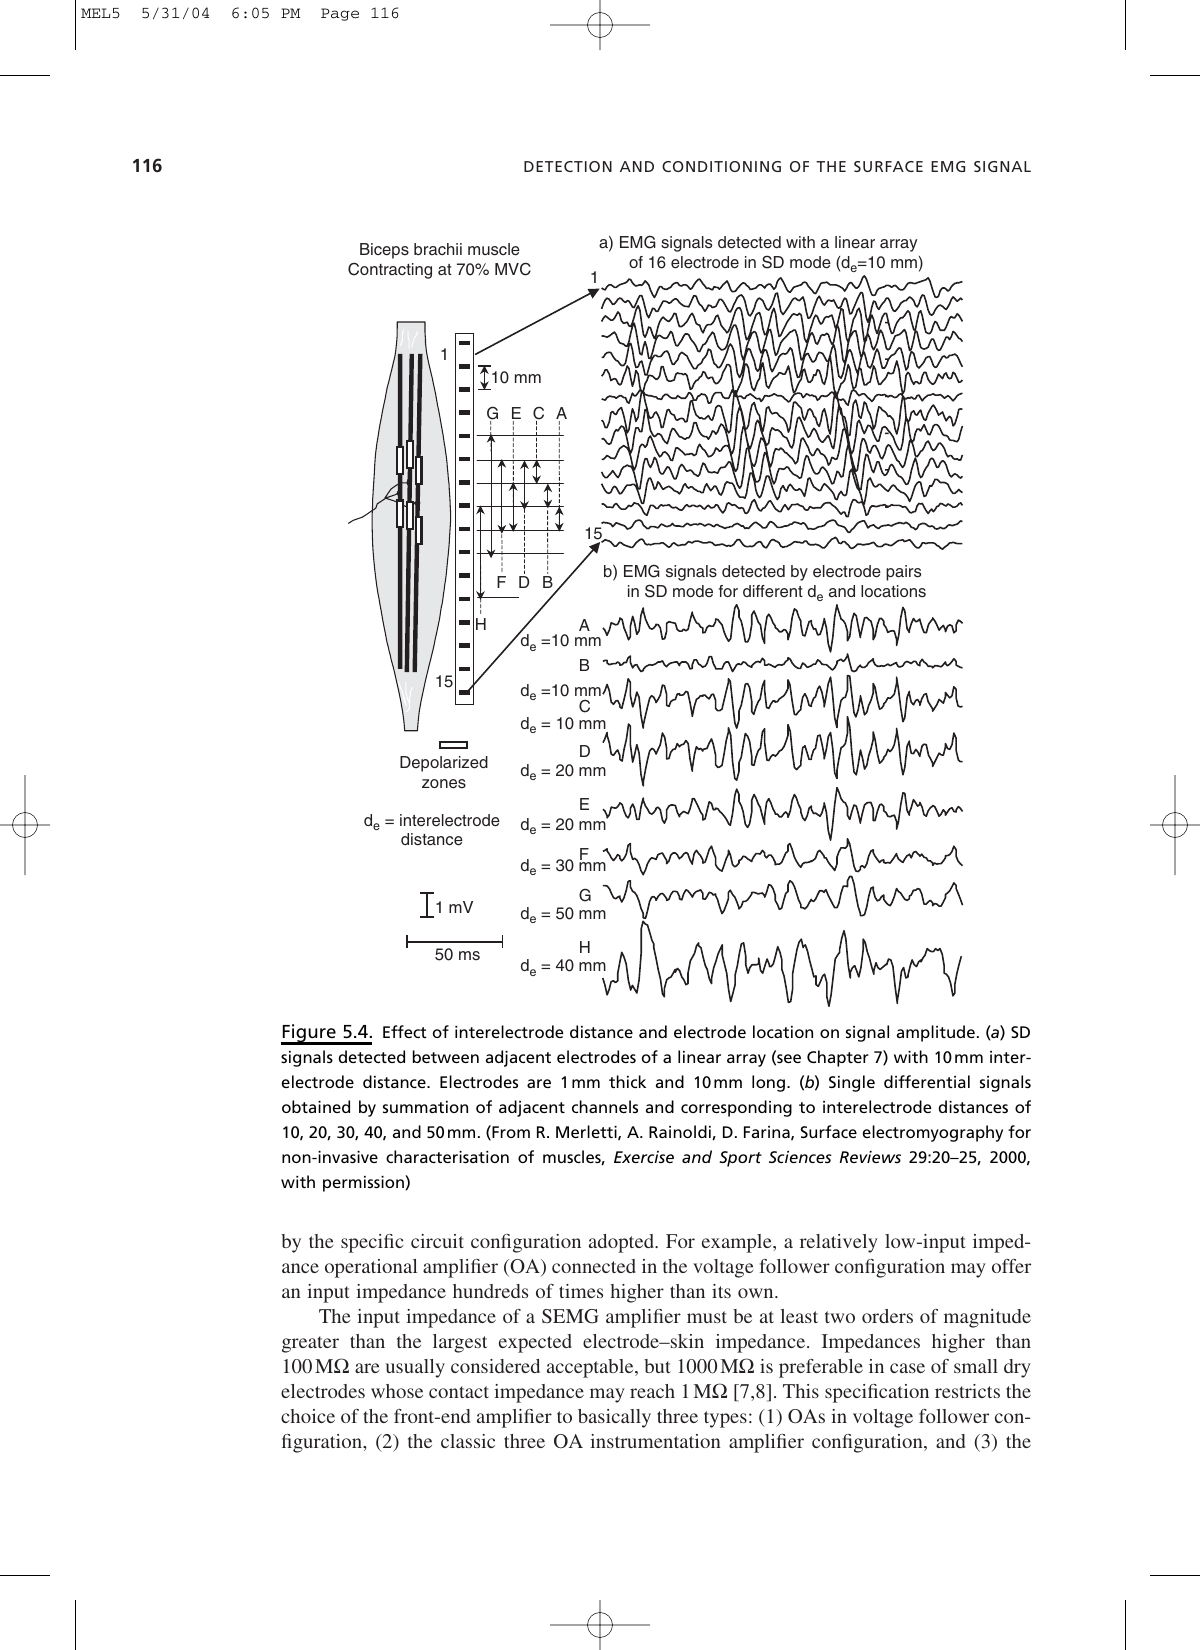
\includegraphics[width=0.82\textwidth]{imagenes/captura_merletti_sec5_5-137.png}
\caption{Página 116 del tratado de Merletti y Parker (2004). Justificación física de los órdenes de magnitud requeridos para la impedancia de entrada.}
\label{fig:merletti_p116}
\end{figure}

\subsection{Modelado de Acoplamiento y Redes de Entrada}
La página 117 detalla la circuitería equivalente de acoplo de entrada, las capacidades parásitas de los cables y la necesidad de drenar las corrientes de polarización hacia masa sin degradar la impedancia vista por el electrodo.

\begin{figure}[htbp]
\centering
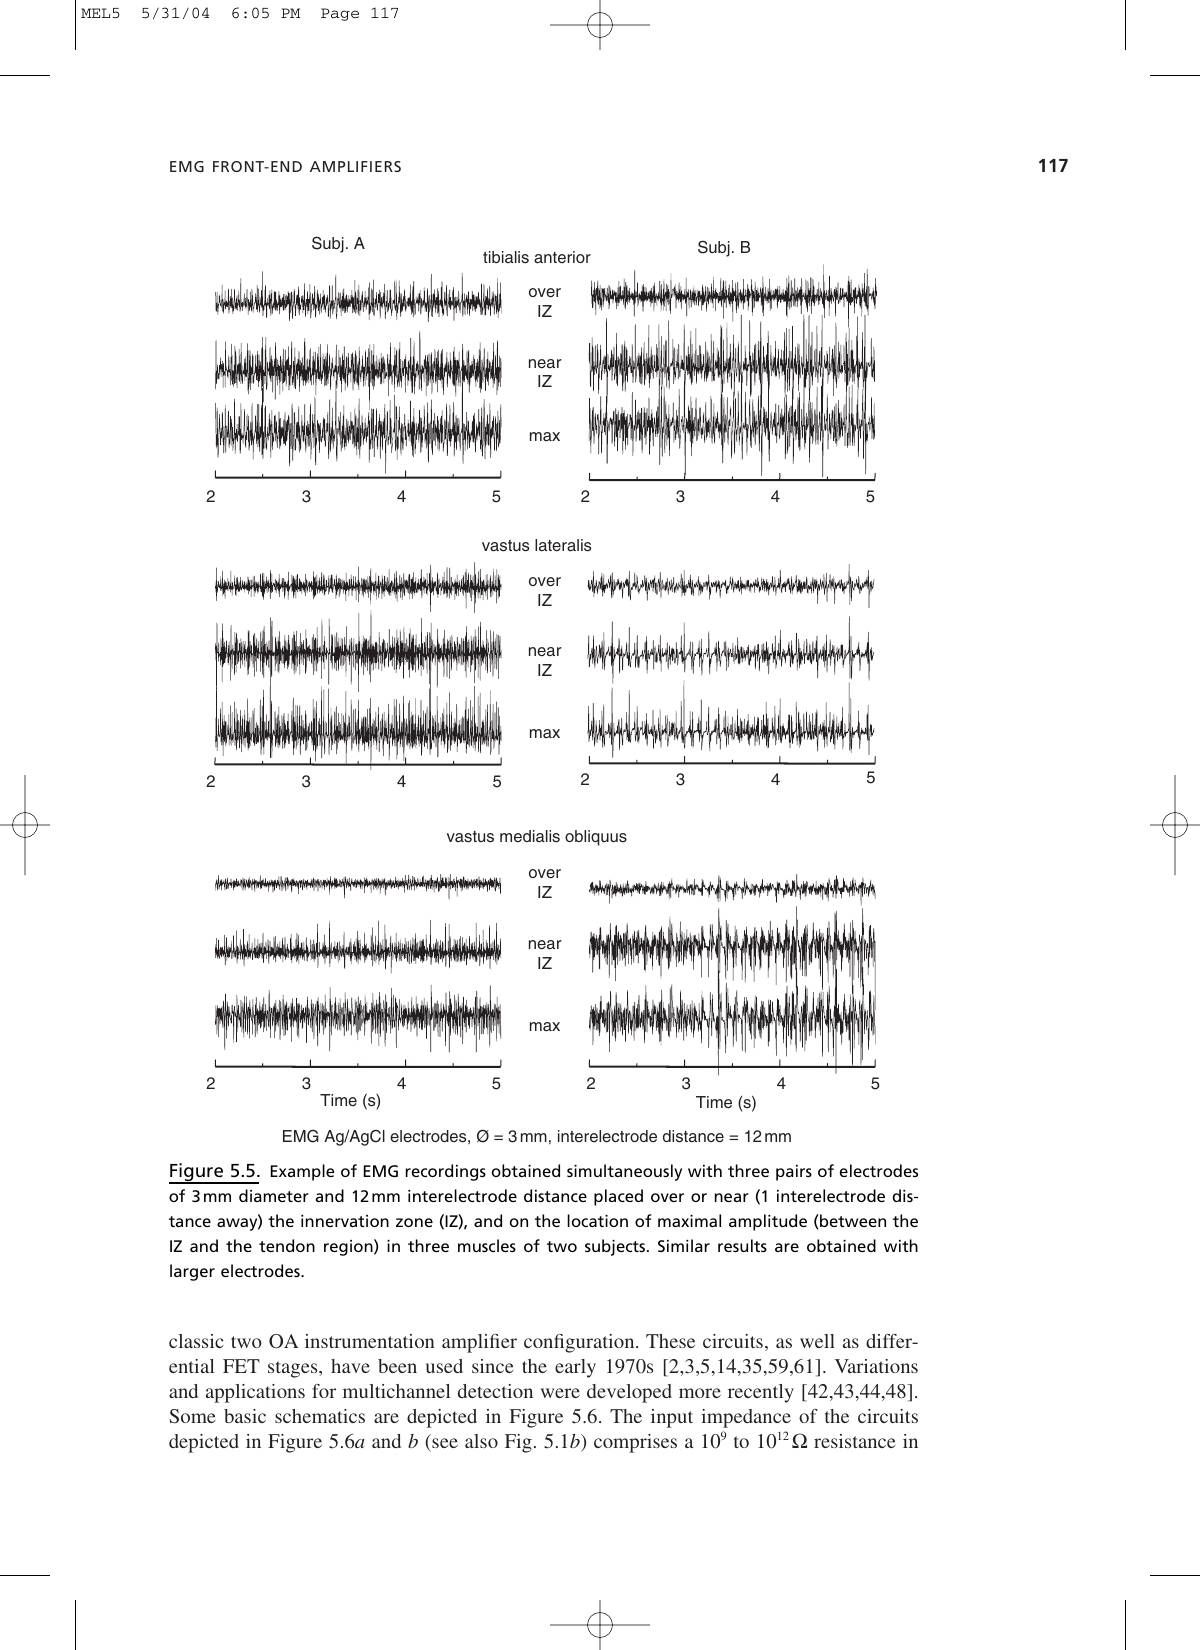
\includegraphics[width=0.82\textwidth]{imagenes/captura_merletti_sec5_5-138.png}
\caption{Página 117 del tratado de Merletti y Parker (2004). Modelado circuital de la interfaz de entrada y acoplamiento capacitivo.}
\label{fig:merletti_p117}
\end{figure}

\subsection{Desacoplo en el Lazo de Ganancia y Desbalance de Electrodos}
La página 118 incluye la fundamental \textbf{Figura 5.6(b)}, donde se ilustra el desacoplo de alterna mediante capacitor serie en la rama de ganancia ($R_G + C_G$), así como la demostración analítica de la ecuación de interferencia de modo común por desbalance $\Delta Z / Z_i$.

\begin{figure}[htbp]
\centering
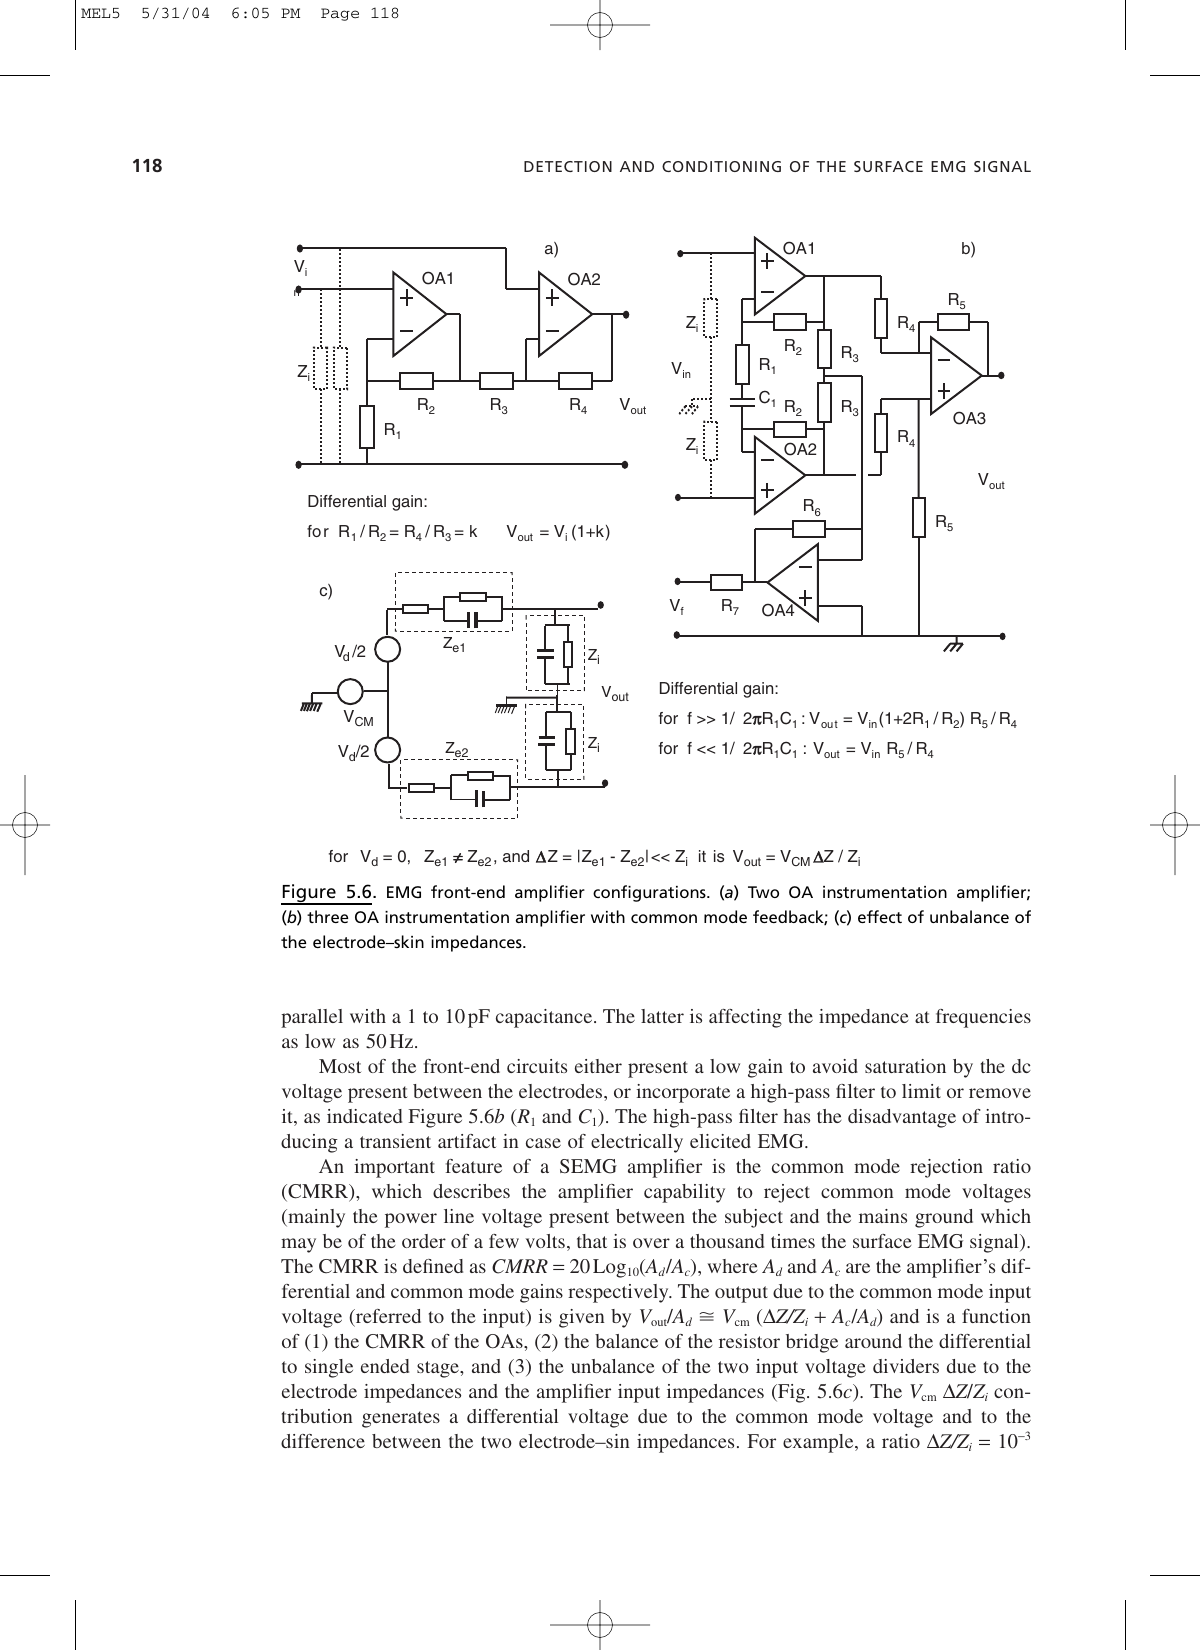
\includegraphics[width=0.82\textwidth]{imagenes/captura_merletti_sec5_5-139.png}
\caption{Página 118 del tratado de Merletti y Parker (2004). Figura 5.6: esquemas circuitales con acoplo en alterna en el lazo de ganancia y deducción de la conversión de modo común a diferencial.}
\label{fig:merletti_p118}
\end{figure}

\subsection{Cuadro de Recomendaciones Oficiales SENIAM}
La página 127 presenta la \textbf{Tabla 5.4} con las recomendaciones oficiales consensuadas por el consorcio europeo SENIAM para sensores, amplificadores de instrumentación y convertidores A/D en electromiografía de superficie.

\begin{figure}[htbp]
\centering
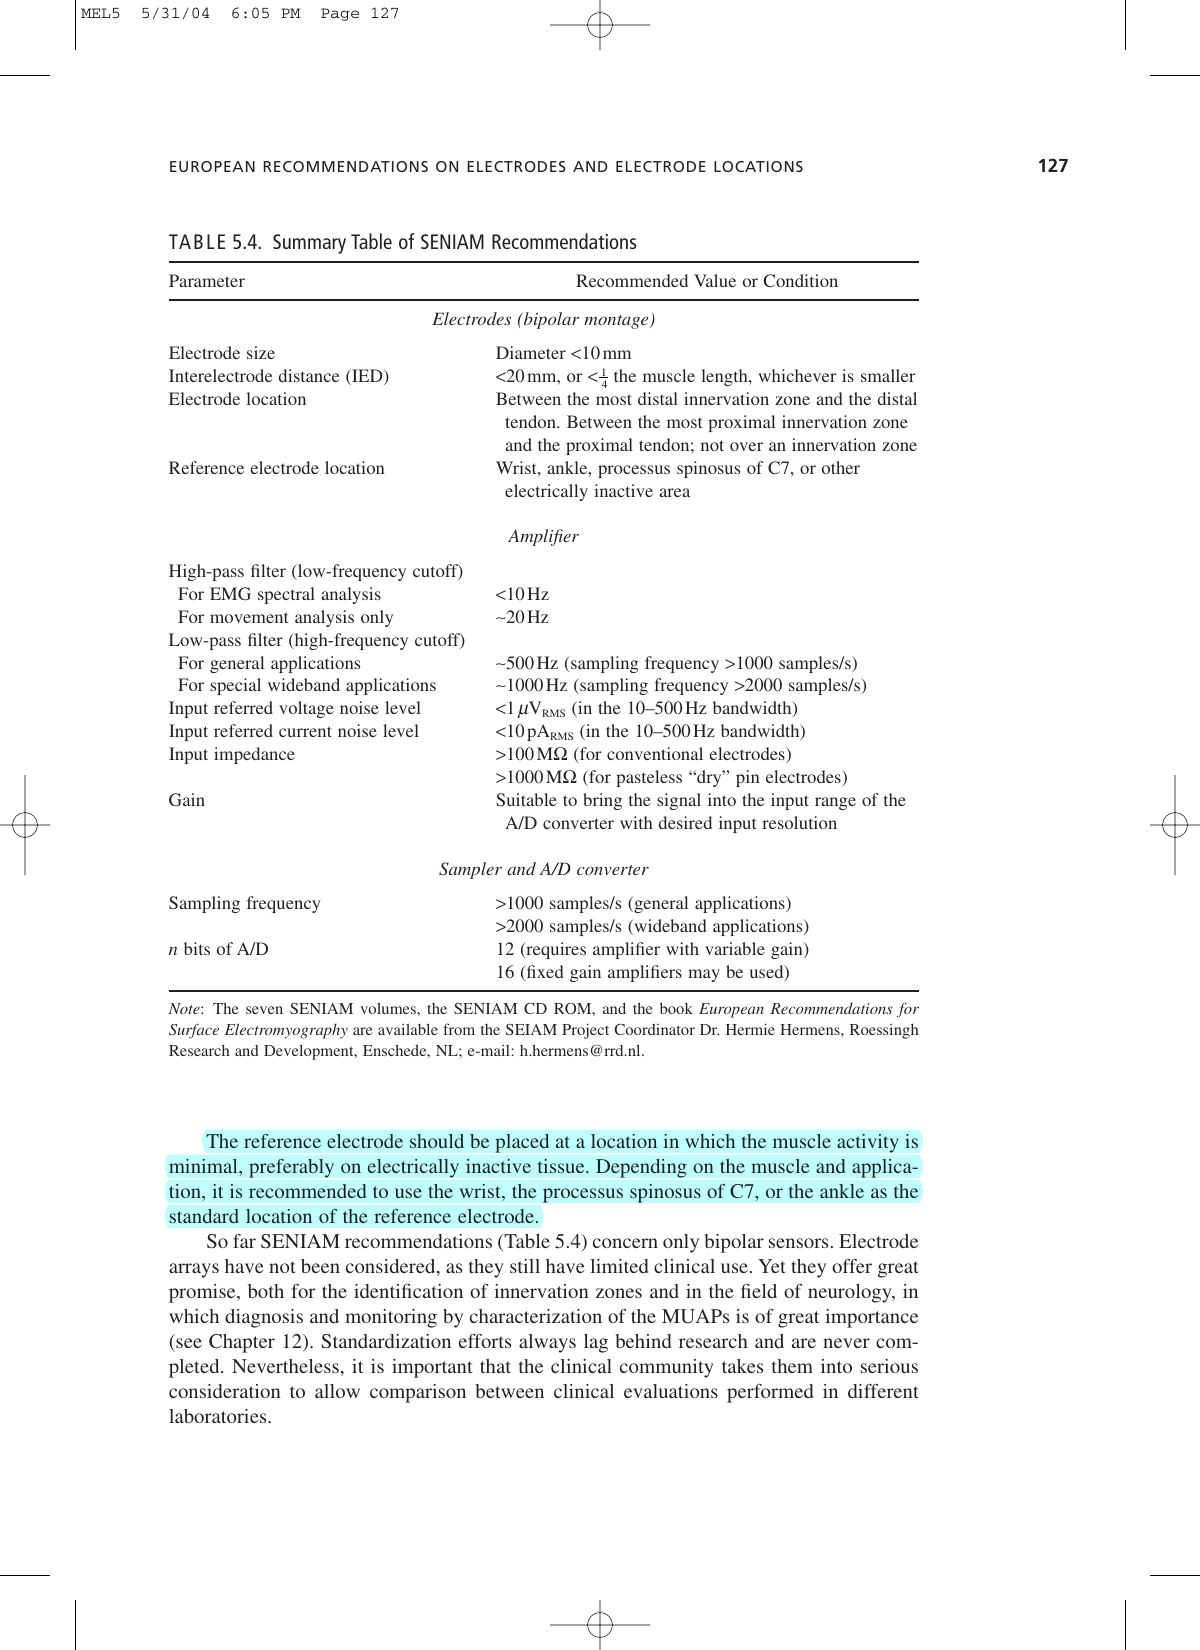
\includegraphics[width=0.82\textwidth]{imagenes/captura_merletti_tabla_seniam-148.png}
\caption{Página 127 del tratado de Merletti y Parker (2004). Tabla 5.4: Cuadro normativo SENIAM para amplificadores sEMG.}
\label{fig:merletti_seniam_p127}
\end{figure}

% ====================================================================
\section{Caracterización Experimental y Circuito Físico Completo}
% ====================================================================

En esta sección se documenta el hardware completo desarrollado por Santiago Prado Rodríguez y Lucas Gastón Braunstein para el Laboratorio de Sistemas Dinámicos, integrando la etapa activa de protección de alimentación, el circuito impreso, la nómina de componentes y la caracterización experimental de ganancia en función de la frecuencia.

\subsection{Esquema Electrónico Integral y Etapa de Alimentación}
La Figura \ref{fig:esquema_proteccion_inf} presenta la etapa de alimentación y protección activa contra inversión de polaridad implementada en el hardware físico. La Figura \ref{fig:esquema_canal_original_inf} detalla el esquema circuital del canal de instrumentación analógico típico basado en el amplificador AD620 (idéntico para los tres canales del sistema).

\begin{figure}[H]
\centering
\resizebox{0.95\linewidth}{!}{%
\begin{circuitikz}[american, thick, font=\sffamily]
  % Marco de Alimentación y Protección con amplia holgura
  \draw[dashed, draw=blue!60, fill=blue!2, rounded corners] (-2.8, 5.0) rectangle (14.2, -5.0);
  \node[anchor=north west, font=\bfseries\color{blue!70!black}] at (-2.5, 4.6) {ETAPA DE ALIMENTACI\'ON Y PROTECCI\'ON ACTIVA $\pm 9\,\text{V}$};

  % Bornera BAT TBLOCK-M3
  \draw (-2.2, 3.6) rectangle (0.6, -3.6);
  \node[font=\bfseries] at (-0.8, 3.0) {BAT};
  \node[font=\scriptsize, anchor=west] at (-2.0, 2.4) {Pin 1: +9V};
  \node[font=\scriptsize, anchor=west] at (-2.0, 0.0) {Pin 2: GND};
  \node[font=\scriptsize, anchor=west] at (-2.0, -2.4) {Pin 3: -9V};
  \draw (0.6, 2.4) -- (1.8, 2.4);
  \draw (0.6, 0.0) -- (1.2, 0.0) node[ground]{};
  \draw (0.6, -2.4) -- (1.8, -2.4);

  % Bornera SWITCH TBLOCK-M4
  \draw (1.8, 3.6) rectangle (4.0, -3.6);
  \node[font=\bfseries] at (2.9, 3.0) {SWITCH};
  \node[font=\scriptsize] at (2.2, 2.4) {1}; \node[font=\scriptsize] at (3.6, 2.4) {2};
  \node[font=\scriptsize] at (2.2, -2.4) {3}; \node[font=\scriptsize] at (3.6, -2.4) {4};
  \draw[very thick] (2.4, 2.4) -- (3.4, 2.4);
  \draw[very thick] (2.4, -2.4) -- (3.4, -2.4);

  % Rieles y Fusibles
  \draw (4.0, 2.4) to[fuse, *-*, l={\small $\text{FUSP} = 0.25\,\text{A}$}] (6.2, 2.4);
  \draw (4.0, -2.4) to[fuse, *-*, l_={\small $\text{FUSN} = 0.25\,\text{A}$}] (6.2, -2.4);

  % --- RIEL POSITIVO (+9V) ---
  % Transistor PMOS F9540N
  \draw (6.2, 2.4) -- (7.5, 2.4) coordinate (s_pos)
        node[pmos, rotate=90, yscale=-1, anchor=S] (QP) {};
  \node[above=6pt, font=\small\bfseries] at (7.5, 2.7) {F9540N};
  \draw (QP.D) -- (13.2, 2.4) node[circle, fill, inner sep=2pt]{} 
        node[right, font=\bfseries\color{red!70!black}] {+9V};

  % Línea de Gate PMOS a y = 1.4
  \draw (QP.G) -- (7.5, 1.4) coordinate (g_pos) -- (9.4, 1.4);

  % Zener D2 entre Gate y Source (en x = 8.4)
  \draw (8.4, 2.4) to[zD, *-, l_={\small $D_2$}] (8.4, 1.4) node[circ]{};

  % Resistencia R3 de Gate a masa (en x = 9.4)
  \draw (9.4, 1.4) to[R, *-, l={\small $R_3 = 10\,\text{k}\Omega$}] (9.4, 0.0);

  % --- RIEL NEGATIVO (-9V) ---
  % Transistor NMOS IRFZ44N
  \draw (6.2, -2.4) -- (7.5, -2.4) coordinate (s_neg)
        node[nmos, rotate=-90, yscale=-1, anchor=S] (QN) {};
  \node[below=6pt, font=\small\bfseries] at (7.5, -2.7) {IRFZ44N};
  \draw (QN.D) -- (13.2, -2.4) node[circle, fill, inner sep=2pt]{} 
        node[right, font=\bfseries\color{blue!70!black}] {-9V};

  % Línea de Gate NMOS a y = -1.4
  \draw (QN.G) -- (7.5, -1.4) coordinate (g_neg) -- (10.6, -1.4);

  % Zener D1 entre Gate y Source (en x = 8.4)
  \draw (8.4, -2.4) to[zD, *-, l={\small $D_1$}] (8.4, -1.4) node[circ]{};

  % Resistencia R1 de Gate a masa (en x = 10.6) con etiqueta a la IZQUIERDA
  \draw (10.6, -1.4) to[R, *-, l={\small $R_1 = 10\,\text{k}\Omega$}] (10.6, 0.0);

  % Resistencias Bleeder (R4 y R2 a masa en x = 12.0)
  \draw (12.0, 2.4) to[R, *-, l={\small $R_4 = 100\,\text{k}\Omega$}] (12.0, 0.0);
  \draw (12.0, -2.4) to[R, *-, l_={\small $R_2 = 100\,\text{k}\Omega$}] (12.0, 0.0);

  % Línea central de masa GND conectando R3, R1, R4, R2
  \draw (7.0, 0.0) node[ground]{} -- (13.2, 0.0) node[circle, fill, inner sep=2pt]{} 
        node[right, font=\bfseries] {GND};
  \draw (9.4, 0.0) node[circ]{};
  \draw (10.6, 0.0) node[circ]{};
  \draw (12.0, 0.0) node[circ]{};

\end{circuitikz}%
}
\caption{Etapa de alimentación y protección activa contra inversión de polaridad $\pm 9\,\text{V}$. Utiliza MOSFETs de canal P (F9540N) y canal N (IRFZ44N) referenciados a tierra para lograr conducción casi ideal ($V_{DS} < 6\,\text{mV}$), diodos Zener 1N4741A ($11\,\text{V}$) y fusibles independientes de $0.25\,\text{A}$.}
\label{fig:esquema_proteccion_inf}
\end{figure}

\begin{figure}[H]
\centering
\resizebox{0.88\linewidth}{!}{%
\begin{circuitikz}[american, thick, font=\sffamily]

    % Marco delimitador con amplia holgura
    \draw[dashed, draw=blue!60, fill=blue!2, rounded corners] (-7.5, 4.6) rectangle (4.8, -4.6);
    \node[anchor=north west, font=\bfseries\color{blue!70!black}] at (-7.2, 4.2) {CANAL T\'IPICO DE INSTRUMENTACI\'ON AD620: TOPOLOG\'IA ORIGINAL};

    % AD620
    \draw[thick] (-0.6, 1.8) -- (2.6, 0) -- (-0.6, -1.8) -- cycle;
    \node at (0.9, 0) {\Large AD620};
    \node at (-0.2, 1.2) {\Large \(-\)};
    \node at (-0.2, -1.2) {\Large \(+\)};

    % Pines de Alimentación (±9V) y Referencia
    \draw[-latex] (0.4, 1.2) -- ++(0, 1.0) node[above, font=\small\bfseries\color{red!70!black}] {+9V};
    \node[left=1pt, font=\scriptsize] at (0.4, 1.4) {7};

    \draw[-latex] (0.4, -1.2) -- ++(0, -1.0) node[below, font=\small\bfseries\color{blue!70!black}] {-9V};
    \node[left=1pt, font=\scriptsize] at (0.4, -1.4) {4};

    \draw (1.4, -0.7) -- ++(0, -1.0) node[ground]{};
    \node[right=2pt, font=\scriptsize] at (1.4, -0.7) {5};

    \draw (2.6, 0) -- ++(1.4, 0) node[ocirc]{} node[pos=0.6, above, font=\scriptsize] {6} 
          node[right, font=\small\bfseries] {$V_{\text{out}}$};

    % Pines 1 y 8 (Resistencia RG = 100 Ohm soldada en placa)
    \draw (-0.6, 0.5) node[right=2pt, font=\scriptsize] {1} -- (-2.2, 0.5) coordinate (r_top);
    \draw (-0.6, -0.5) node[right=2pt, font=\scriptsize] {8} -- (-2.2, -0.5) coordinate (r_bot);
    \draw (r_top) to[R, l_={\small $R_G = 100\,\Omega$}, *-*] (r_bot);

    % Entradas con Filtro RC (33 nF + 100 k)
    % Línea Vin-
    \draw (-6.8, 1.3) node[left, font=\small\bfseries] {\(V_{\mathrm{in}}^-\)}
          to[C, l={\small $33\text{ nF}$}] (-4.2, 1.3) coordinate (juncA)
          -- (-0.6, 1.3) node[pos=0.8, above=1pt, font=\scriptsize] {2};
    % Resistencia 100k hacia GND en y = 2.6 con etiqueta a la DERECHA (l_)
    \draw (juncA) to[R, *-, l_={\small $100\text{ k}\Omega$}] (-4.2, 2.6) node[ground, yscale=-1]{};

    % Línea Vin+
    \draw (-6.8, -1.3) node[left, font=\small\bfseries] {\(V_{\mathrm{in}}^+\)}
          to[C, l_={\small $33\text{ nF}$}] (-4.2, -1.3) coordinate (juncB)
          -- (-0.6, -1.3) node[pos=0.8, below=1pt, font=\scriptsize] {3};
    % Resistencia 100k hacia GND en y = -2.6 con etiqueta a la DERECHA (l)
    \draw (juncB) to[R, *-, l={\small $100\text{ k}\Omega$}] (-4.2, -2.6) node[ground]{};

\end{circuitikz}%
}
\caption{Canal típico de instrumentación diferencial AD620 en su topología original (idéntico para los 3 canales de la placa). Dispone de un filtro pasa-altos pasivo unipolar a la entrada ($C = 33\,\text{nF}$, $R = 100\,\text{k}\Omega$, $f_c \approx 48.23\,\text{Hz}$) y resistencia de ganancia fija soldada en placa $R_G = 100\,\Omega$ ($G \approx 495\,\text{V/V}$).}
\label{fig:esquema_canal_original_inf}
\end{figure}

\begin{figure}[H]
\centering
\resizebox{\linewidth}{!}{%
\begin{circuitikz}[american, thick, font=\sffamily]

  % ====================================================
  % BLOQUE 1: ALIMENTACION Y PROTECCION ACTIVA (IZQUIERDA)
  % ====================================================
  \begin{scope}[xshift=-14cm, yshift=0cm]
    \draw[dashed, draw=blue!60, fill=blue!2, rounded corners] (-2.8, 9.2) rectangle (13.6, -9.2);
    \node[anchor=north west, font=\bfseries\color{blue!70!black}] at (-2.5, 8.8) {ETAPA DE ALIMENTACI\'ON Y PROTECCI\'ON ACTIVA $\pm 9\,\text{V}$};

    % Bornera BAT TBLOCK-M3
    \draw (-2.2, 5.0) rectangle (0.4, -5.0);
    \node[font=\bfseries] at (-0.9, 4.4) {BAT};
    \node[font=\scriptsize, anchor=west] at (-2.0, 3.4) {Pin 1: +9V};
    \node[font=\scriptsize, anchor=west] at (-2.0, 0.0) {Pin 2: GND};
    \node[font=\scriptsize, anchor=west] at (-2.0, -3.4) {Pin 3: -9V};
    \draw (0.4, 3.4) -- (1.6, 3.4);
    \draw (0.4, 0.0) -- (1.0, 0.0) node[ground]{};
    \draw (0.4, -3.4) -- (1.6, -3.4);

    % Bornera SWITCH TBLOCK-M4
    \draw (1.6, 5.0) rectangle (3.8, -5.0);
    \node[font=\bfseries] at (2.7, 4.4) {SWITCH};
    \node[font=\scriptsize] at (2.0, 3.4) {1}; \node[font=\scriptsize] at (3.4, 3.4) {2};
    \node[font=\scriptsize] at (2.0, -3.4) {3}; \node[font=\scriptsize] at (3.4, -3.4) {4};
    \draw[very thick] (2.2, 3.4) -- (3.2, 3.4);
    \draw[very thick] (2.2, -3.4) -- (3.2, -3.4);

    % Fusibles
    \draw (3.8, 3.4) to[fuse, *-*, l={\small $\text{FUSP} = 0.25\,\text{A}$}] (6.0, 3.4);
    \draw (3.8, -3.4) to[fuse, *-*, l_={\small $\text{FUSN} = 0.25\,\text{A}$}] (6.0, -3.4);

    % --- RIEL POSITIVO (+9V) ---
    \draw (6.0, 3.4) -- (7.2, 3.4) coordinate (s_pos)
          node[pmos, rotate=90, yscale=-1, anchor=S] (QP) {};
    \node[above=6pt, font=\small\bfseries] at (7.2, 3.7) {F9540N};
    \draw (QP.D) -- (12.2, 3.4) node[circle, fill, inner sep=2pt]{} 
          node[right, font=\bfseries\color{red!70!black}] {+9V};

    \draw (QP.G) -- (7.2, 1.8) coordinate (g_pos) -- (9.2, 1.8);
    \draw (8.0, 3.4) to[zD, *-, l_={\small $D_2$}] (8.0, 1.8) node[circ]{};
    \draw (9.2, 1.8) to[R, *-, l={\small $R_3 = 10\,\text{k}\Omega$}] (9.2, 0.0);

    % --- RIEL NEGATIVO (-9V) ---
    \draw (6.0, -3.4) -- (7.2, -3.4) coordinate (s_neg)
          node[nmos, rotate=-90, yscale=-1, anchor=S] (QN) {};
    \node[below=6pt, font=\small\bfseries] at (7.2, -3.7) {IRFZ44N};
    \draw (QN.D) -- (12.2, -3.4) node[circle, fill, inner sep=2pt]{} 
          node[right, font=\bfseries\color{blue!70!black}] {-9V};

    \draw (QN.G) -- (7.2, -1.8) coordinate (g_neg) -- (10.2, -1.8);
    \draw (8.0, -3.4) to[zD, *-, l={\small $D_1$}] (8.0, -1.8) node[circ]{};
    \draw (10.2, -1.8) to[R, *-, l={\small $R_1 = 10\,\text{k}\Omega$}] (10.2, 0.0);

    % Resistencias Bleeder
    \draw (11.2, 3.4) to[R, *-, l_={\small $R_4 = 100\,\text{k}\Omega$}] (11.2, 0.0);
    \draw (11.2, -3.4) to[R, *-, l={\small $R_2 = 100\,\text{k}\Omega$}] (11.2, 0.0);

    % Masa GND
    \draw (6.8, 0.0) node[ground]{} -- (12.2, 0.0) node[circle, fill, inner sep=2pt]{} 
          node[right, font=\bfseries] {GND};
    \draw (9.2, 0.0) node[circ]{};
    \draw (10.2, 0.0) node[circ]{};
    \draw (11.2, 0.0) node[circ]{};
  \end{scope}

  % ====================================================
  % BLOQUE 2: CANAL 1 (U1 - AD620)
  % ====================================================
  \begin{scope}[xshift=4.8cm, yshift=6.0cm]
    \draw[dashed, draw=blue!60, fill=blue!2, rounded corners] (-3.8, 2.8) rectangle (9.6, -2.8);
    \node[anchor=north west, font=\bfseries\color{blue!70!black}] at (-3.5, 2.5) {CANAL 1};

    % Bornera IN1
    \draw (-3.4, 1.3) rectangle (-2.0, -1.3);
    \node[font=\bfseries\scriptsize] at (-2.7, 0.9) {IN1};
    \node[font=\tiny] at (-3.1, 0.45) {1}; \draw (-2.0, 0.45) -- (-1.6, 0.45) node[ground]{};
    \node[font=\tiny] at (-3.1, 0.0) {2};  \draw (-2.0, 0.0) -- (-1.0, 0.0) -- (-1.0, 0.9) coordinate (in1_neg_start);
    \node[font=\tiny] at (-3.1, -0.45) {3}; \draw (-2.0, -0.45) -- (-1.0, -0.45) -- (-1.0, -0.9) coordinate (in1_pos_start);

    % Filtros de entrada
    \draw (in1_neg_start) to[C, l={\scriptsize $C_2 = 33\,\text{nF}$}] (0.8, 0.9) coordinate (junc1_neg) -- (3.0, 0.9);
    \draw (junc1_neg) to[R, *-, l_={\scriptsize $R_2 = 100\,\text{k}\Omega$}] (0.8, 1.7) node[ground, yscale=-1]{};

    \draw (in1_pos_start) to[C, l_={\scriptsize $C_1 = 33\,\text{nF}$}] (0.8, -0.9) coordinate (junc1_pos) -- (3.0, -0.9);
    \draw (junc1_pos) to[R, *-, l={\scriptsize $R_1 = 100\,\text{k}\Omega$}] (0.8, -1.7) node[ground]{};

    % AD620 (U1)
    \draw[thick] (3.0, 1.4) -- (5.4, 0.0) -- (3.0, -1.4) -- cycle;
    \node at (4.1, 0.0) {\small AD620};
    \node[below=4pt, font=\tiny] at (4.1, 0.0) {U1};
    \node at (3.3, 0.9) {\scriptsize \(-\)};
    \node at (3.3, -0.9) {\scriptsize \(+\)};

    % Resistencia de ganancia RG (Pin 1 y 8)
    \draw (3.0, 0.4) node[right=1pt, font=\tiny] {1} -- (2.2, 0.4) coordinate (rg1_top);
    \draw (3.0, -0.4) node[right=1pt, font=\tiny] {8} -- (2.2, -0.4) coordinate (rg1_bot);
    \draw (rg1_top) to[R, *-*, l_={\scriptsize $R_3 = 100\,\Omega$}] (rg1_bot);

    % Alimentación U1
    \draw (3.8, 0.9) -- ++(0, 0.7) node[above, font=\tiny\bfseries\color{red!70!black}] {+9V};
    \draw (3.8, -0.9) -- ++(0, -0.7) node[below, font=\tiny\bfseries\color{blue!70!black}] {-9V};
    \draw (4.6, -0.5) -- ++(0, -0.7) node[ground]{};

    % Salida y Bornera OUT1
    \draw (5.4, 0.0) -- (7.6, 0.0) coordinate (out1_wire);
    \draw (7.6, 1.0) rectangle (9.2, -1.0);
    \node[font=\bfseries\scriptsize] at (8.4, 0.6) {OUT1};
    \node[font=\tiny] at (8.0, 0.0) {2}; \draw (out1_wire) -- (7.6, 0.0);
    \node[font=\tiny] at (8.0, -0.5) {1}; \draw (9.2, -0.5) -- ++(0.3, 0) node[ground]{};
  \end{scope}

  % ====================================================
  % BLOQUE 3: CANAL 2 (U2 - AD620)
  % ====================================================
  \begin{scope}[xshift=4.8cm, yshift=0.0cm]
    \draw[dashed, draw=blue!60, fill=blue!2, rounded corners] (-3.8, 2.8) rectangle (9.6, -2.8);
    \node[anchor=north west, font=\bfseries\color{blue!70!black}] at (-3.5, 2.5) {CANAL 2};

    % Bornera IN2
    \draw (-3.4, 1.3) rectangle (-2.0, -1.3);
    \node[font=\bfseries\scriptsize] at (-2.7, 0.9) {IN2};
    \node[font=\tiny] at (-3.1, 0.45) {1}; \draw (-2.0, 0.45) -- (-1.6, 0.45) node[ground]{};
    \node[font=\tiny] at (-3.1, 0.0) {2};  \draw (-2.0, 0.0) -- (-1.0, 0.0) -- (-1.0, 0.9) coordinate (in2_neg_start);
    \node[font=\tiny] at (-3.1, -0.45) {3}; \draw (-2.0, -0.45) -- (-1.0, -0.45) -- (-1.0, -0.9) coordinate (in2_pos_start);

    % Filtros de entrada
    \draw (in2_neg_start) to[C, l={\scriptsize $C_4 = 33\,\text{nF}$}] (0.8, 0.9) coordinate (junc2_neg) -- (3.0, 0.9);
    \draw (junc2_neg) to[R, *-, l_={\scriptsize $R_4 = 100\,\text{k}\Omega$}] (0.8, 1.7) node[ground, yscale=-1]{};

    \draw (in2_pos_start) to[C, l_={\scriptsize $C_3 = 33\,\text{nF}$}] (0.8, -0.9) coordinate (junc2_pos) -- (3.0, -0.9);
    \draw (junc2_pos) to[R, *-, l={\scriptsize $R_5 = 100\,\text{k}\Omega$}] (0.8, -1.7) node[ground]{};

    % AD620 (U2)
    \draw[thick] (3.0, 1.4) -- (5.4, 0.0) -- (3.0, -1.4) -- cycle;
    \node at (4.1, 0.0) {\small AD620};
    \node[below=4pt, font=\tiny] at (4.1, 0.0) {U2};
    \node at (3.3, 0.9) {\scriptsize \(-\)};
    \node at (3.3, -0.9) {\scriptsize \(+\)};

    % Resistencia de ganancia RG (Pin 1 y 8)
    \draw (3.0, 0.4) node[right=1pt, font=\tiny] {1} -- (2.2, 0.4) coordinate (rg2_top);
    \draw (3.0, -0.4) node[right=1pt, font=\tiny] {8} -- (2.2, -0.4) coordinate (rg2_bot);
    \draw (rg2_top) to[R, *-*, l_={\scriptsize $R_6 = 100\,\Omega$}] (rg2_bot);

    % Alimentación U2
    \draw (3.8, 0.9) -- ++(0, 0.7) node[above, font=\tiny\bfseries\color{red!70!black}] {+9V};
    \draw (3.8, -0.9) -- ++(0, -0.7) node[below, font=\tiny\bfseries\color{blue!70!black}] {-9V};
    \draw (4.6, -0.5) -- ++(0, -0.7) node[ground]{};

    % Salida y Bornera OUT2
    \draw (5.4, 0.0) -- (7.6, 0.0) coordinate (out2_wire);
    \draw (7.6, 1.0) rectangle (9.2, -1.0);
    \node[font=\bfseries\scriptsize] at (8.4, 0.6) {OUT2};
    \node[font=\tiny] at (8.0, 0.0) {2}; \draw (out2_wire) -- (7.6, 0.0);
    \node[font=\tiny] at (8.0, -0.5) {1}; \draw (9.2, -0.5) -- ++(0.3, 0) node[ground]{};
  \end{scope}

  % ====================================================
  % BLOQUE 4: CANAL 3 (U3 - AD620)
  % ====================================================
  \begin{scope}[xshift=4.8cm, yshift=-6.0cm]
    \draw[dashed, draw=blue!60, fill=blue!2, rounded corners] (-3.8, 2.8) rectangle (9.6, -2.8);
    \node[anchor=north west, font=\bfseries\color{blue!70!black}] at (-3.5, 2.5) {CANAL 3};

    % Bornera IN3GND
    \draw (-3.4, 1.3) rectangle (-2.0, -1.3);
    \node[font=\bfseries\scriptsize] at (-2.7, 0.9) {IN3GND};
    \node[font=\tiny] at (-3.1, 0.45) {1}; \draw (-2.0, 0.45) -- (-1.4, 0.45) node[ground]{} node[right=2pt, font=\tiny\bfseries] {REF};
    \node[font=\tiny] at (-3.1, 0.0) {2};  \draw (-2.0, 0.0) -- (-1.0, 0.0) -- (-1.0, 0.9) coordinate (in3_neg_start);
    \node[font=\tiny] at (-3.1, -0.45) {3}; \draw (-2.0, -0.45) -- (-1.0, -0.45) -- (-1.0, -0.9) coordinate (in3_pos_start);

    % Filtros de entrada
    \draw (in3_neg_start) to[C, l={\scriptsize $C_6 = 33\,\text{nF}$}] (0.8, 0.9) coordinate (junc3_neg) -- (3.0, 0.9);
    \draw (junc3_neg) to[R, *-, l_={\scriptsize $R_7 = 100\,\text{k}\Omega$}] (0.8, 1.7) node[ground, yscale=-1]{};

    \draw (in3_pos_start) to[C, l_={\scriptsize $C_5 = 33\,\text{nF}$}] (0.8, -0.9) coordinate (junc3_pos) -- (3.0, -0.9);
    \draw (junc3_pos) to[R, *-, l={\scriptsize $R_8 = 100\,\text{k}\Omega$}] (0.8, -1.7) node[ground]{};

    % AD620 (U3)
    \draw[thick] (3.0, 1.4) -- (5.4, 0.0) -- (3.0, -1.4) -- cycle;
    \node at (4.1, 0.0) {\small AD620};
    \node[below=4pt, font=\tiny] at (4.1, 0.0) {U3};
    \node at (3.3, 0.9) {\scriptsize \(-\)};
    \node at (3.3, -0.9) {\scriptsize \(+\)};

    % Resistencia de ganancia RG (Pin 1 y 8)
    \draw (3.0, 0.4) node[right=1pt, font=\tiny] {1} -- (2.2, 0.4) coordinate (rg3_top);
    \draw (3.0, -0.4) node[right=1pt, font=\tiny] {8} -- (2.2, -0.4) coordinate (rg3_bot);
    \draw (rg3_top) to[R, *-*, l_={\scriptsize $R_9 = 100\,\Omega$}] (rg3_bot);

    % Alimentación U3
    \draw (3.8, 0.9) -- ++(0, 0.7) node[above, font=\tiny\bfseries\color{red!70!black}] {+9V};
    \draw (3.8, -0.9) -- ++(0, -0.7) node[below, font=\tiny\bfseries\color{blue!70!black}] {-9V};
    \draw (4.6, -0.5) -- ++(0, -0.7) node[ground]{};

    % Salida y Bornera OUT3
    \draw (5.4, 0.0) -- (7.6, 0.0) coordinate (out3_wire);
    \draw (7.6, 1.0) rectangle (9.2, -1.0);
    \node[font=\bfseries\scriptsize] at (8.4, 0.6) {OUT3};
    \node[font=\tiny] at (8.0, 0.0) {2}; \draw (out3_wire) -- (7.6, 0.0);
    \node[font=\tiny] at (8.0, -0.5) {1}; \draw (9.2, -0.5) -- ++(0.3, 0) node[ground]{};
  \end{scope}
%
\end{circuitikz}%
}
\caption{Esquema electrónico integral del front-end sEMG de 3 canales. A la izquierda: bloque de alimentación con protección activa contra inversión de polaridad por MOSFETs (F9540N y IRFZ44N), diodos Zener 1N4741A, fusibles de $0.25\,\text{A}$ e interruptor bipolar. A la derecha: los 3 canales de instrumentación diferencial independientes con AD620 (U1, U2, U3) y sus borneras correspondientes (IN1, IN2, IN3GND, OUT1, OUT2, OUT3).}
\label{fig:esquema_completo_3canales_inf}
\end{figure}

El sistema incorpora una etapa de protección activa contra inversión de polaridad que supera las limitaciones de los diodos rectificadores comunes:
\begin{itemize}
    \item \textbf{Riel Negativo ($-9\,\text{V}$):} Utiliza un MOSFET de canal N (\textbf{IRFZ44N}) en el retorno. Con alimentación correcta, la compuerta se referencia a masa a través de $R_1 = 10\,\text{k}\Omega$, fijando $V_{GS} \approx +9\,\text{V}$ y saturando el canal con $R_{DS(\text{on})} \approx 17.5\,\text{m}\Omega$. La caída de tensión es de apenas $1.4\,\text{mV}$ a $50\,\text{mA}$, sin pérdidas térmicas.
    \item \textbf{Riel Positivo ($+9\,\text{V}$):} Utiliza un MOSFET de canal P (\textbf{F9540N}) en serie. Su compuerta referenciada a masa mediante $R_3 = 10\,\text{k}\Omega$ establece $V_{GS} \approx -9\,\text{V}$, conduciendo con $R_{DS(\text{on})} \approx 0.11\,\Omega$ y una caída de tensión de solo $5.5\,\text{mV}$.
    \item \textbf{Protección por Diodos Zener:} Los diodos $D_1$ y $D_2$ (1N4741A, $V_Z = 11\,\text{V}$) fijan la tensión máxima compuerta-fuente, protegiendo el dieléctrico de los transistores ante transitorios de encendido.
    \item \textbf{Fusibles de Acción Rápida:} Las líneas protegidas se conectan a fusibles de $0.25\,\text{A}$ ($FUSE_1$ y $FUSE_2$), previniendo fallos destructivos ante cortocircuitos accidentales.
\end{itemize}

\subsection{Curvas de Amplificación en Función de la Resistencia de Ganancia}
Para contrastar el comportamiento medido en laboratorio frente al modelo físico analítico, la Figura \ref{fig:comparativa_frecuencia_inf} exhibe la respuesta en frecuencia: a la izquierda, las mediciones experimentales con osciloscopio y generador de funciones ($V_{\text{in}} = 2\,\text{mV}_{\text{pp}}$) barriendo frecuencias desde $10\,\text{Hz}$ hasta $100\,\text{kHz}$; a la derecha, la formulación analítica completa del sistema:
\begin{equation}
|H(f)| = \frac{\frac{f}{f_L}}{\sqrt{1 + \left(\frac{f}{f_L}\right)^2}} \cdot \frac{1 + \frac{49.4\,\text{k}\Omega}{R_G}}{\sqrt{1 + \left(\frac{f}{f_H}\right)^2}}
\end{equation}
con $f_L \approx 48.23\,\text{Hz}$ y $f_H \approx \frac{1.2 \times 10^7}{G}\,\text{Hz}$.

\begin{figure}[H]
    \centering
    \begin{subfigure}[b]{0.48\linewidth}
        \centering
        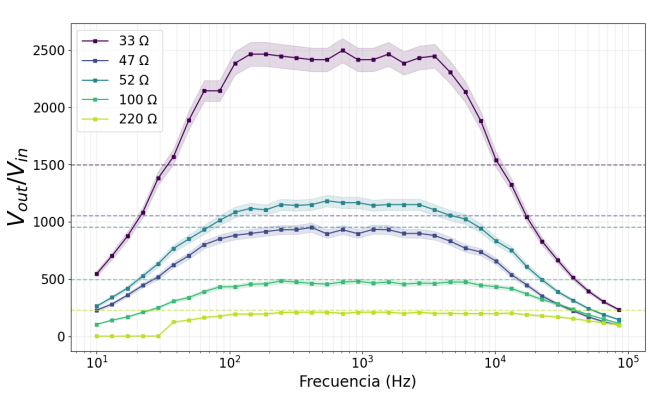
\includegraphics[width=\linewidth]{imagenes/curvas_ganancia_experimental_fig18.png}
        \caption{Medición experimental en laboratorio}
        \label{fig:curvas_experimentales_inf}
    \end{subfigure}
    \hfill
    \begin{subfigure}[b]{0.48\linewidth}
        \centering
        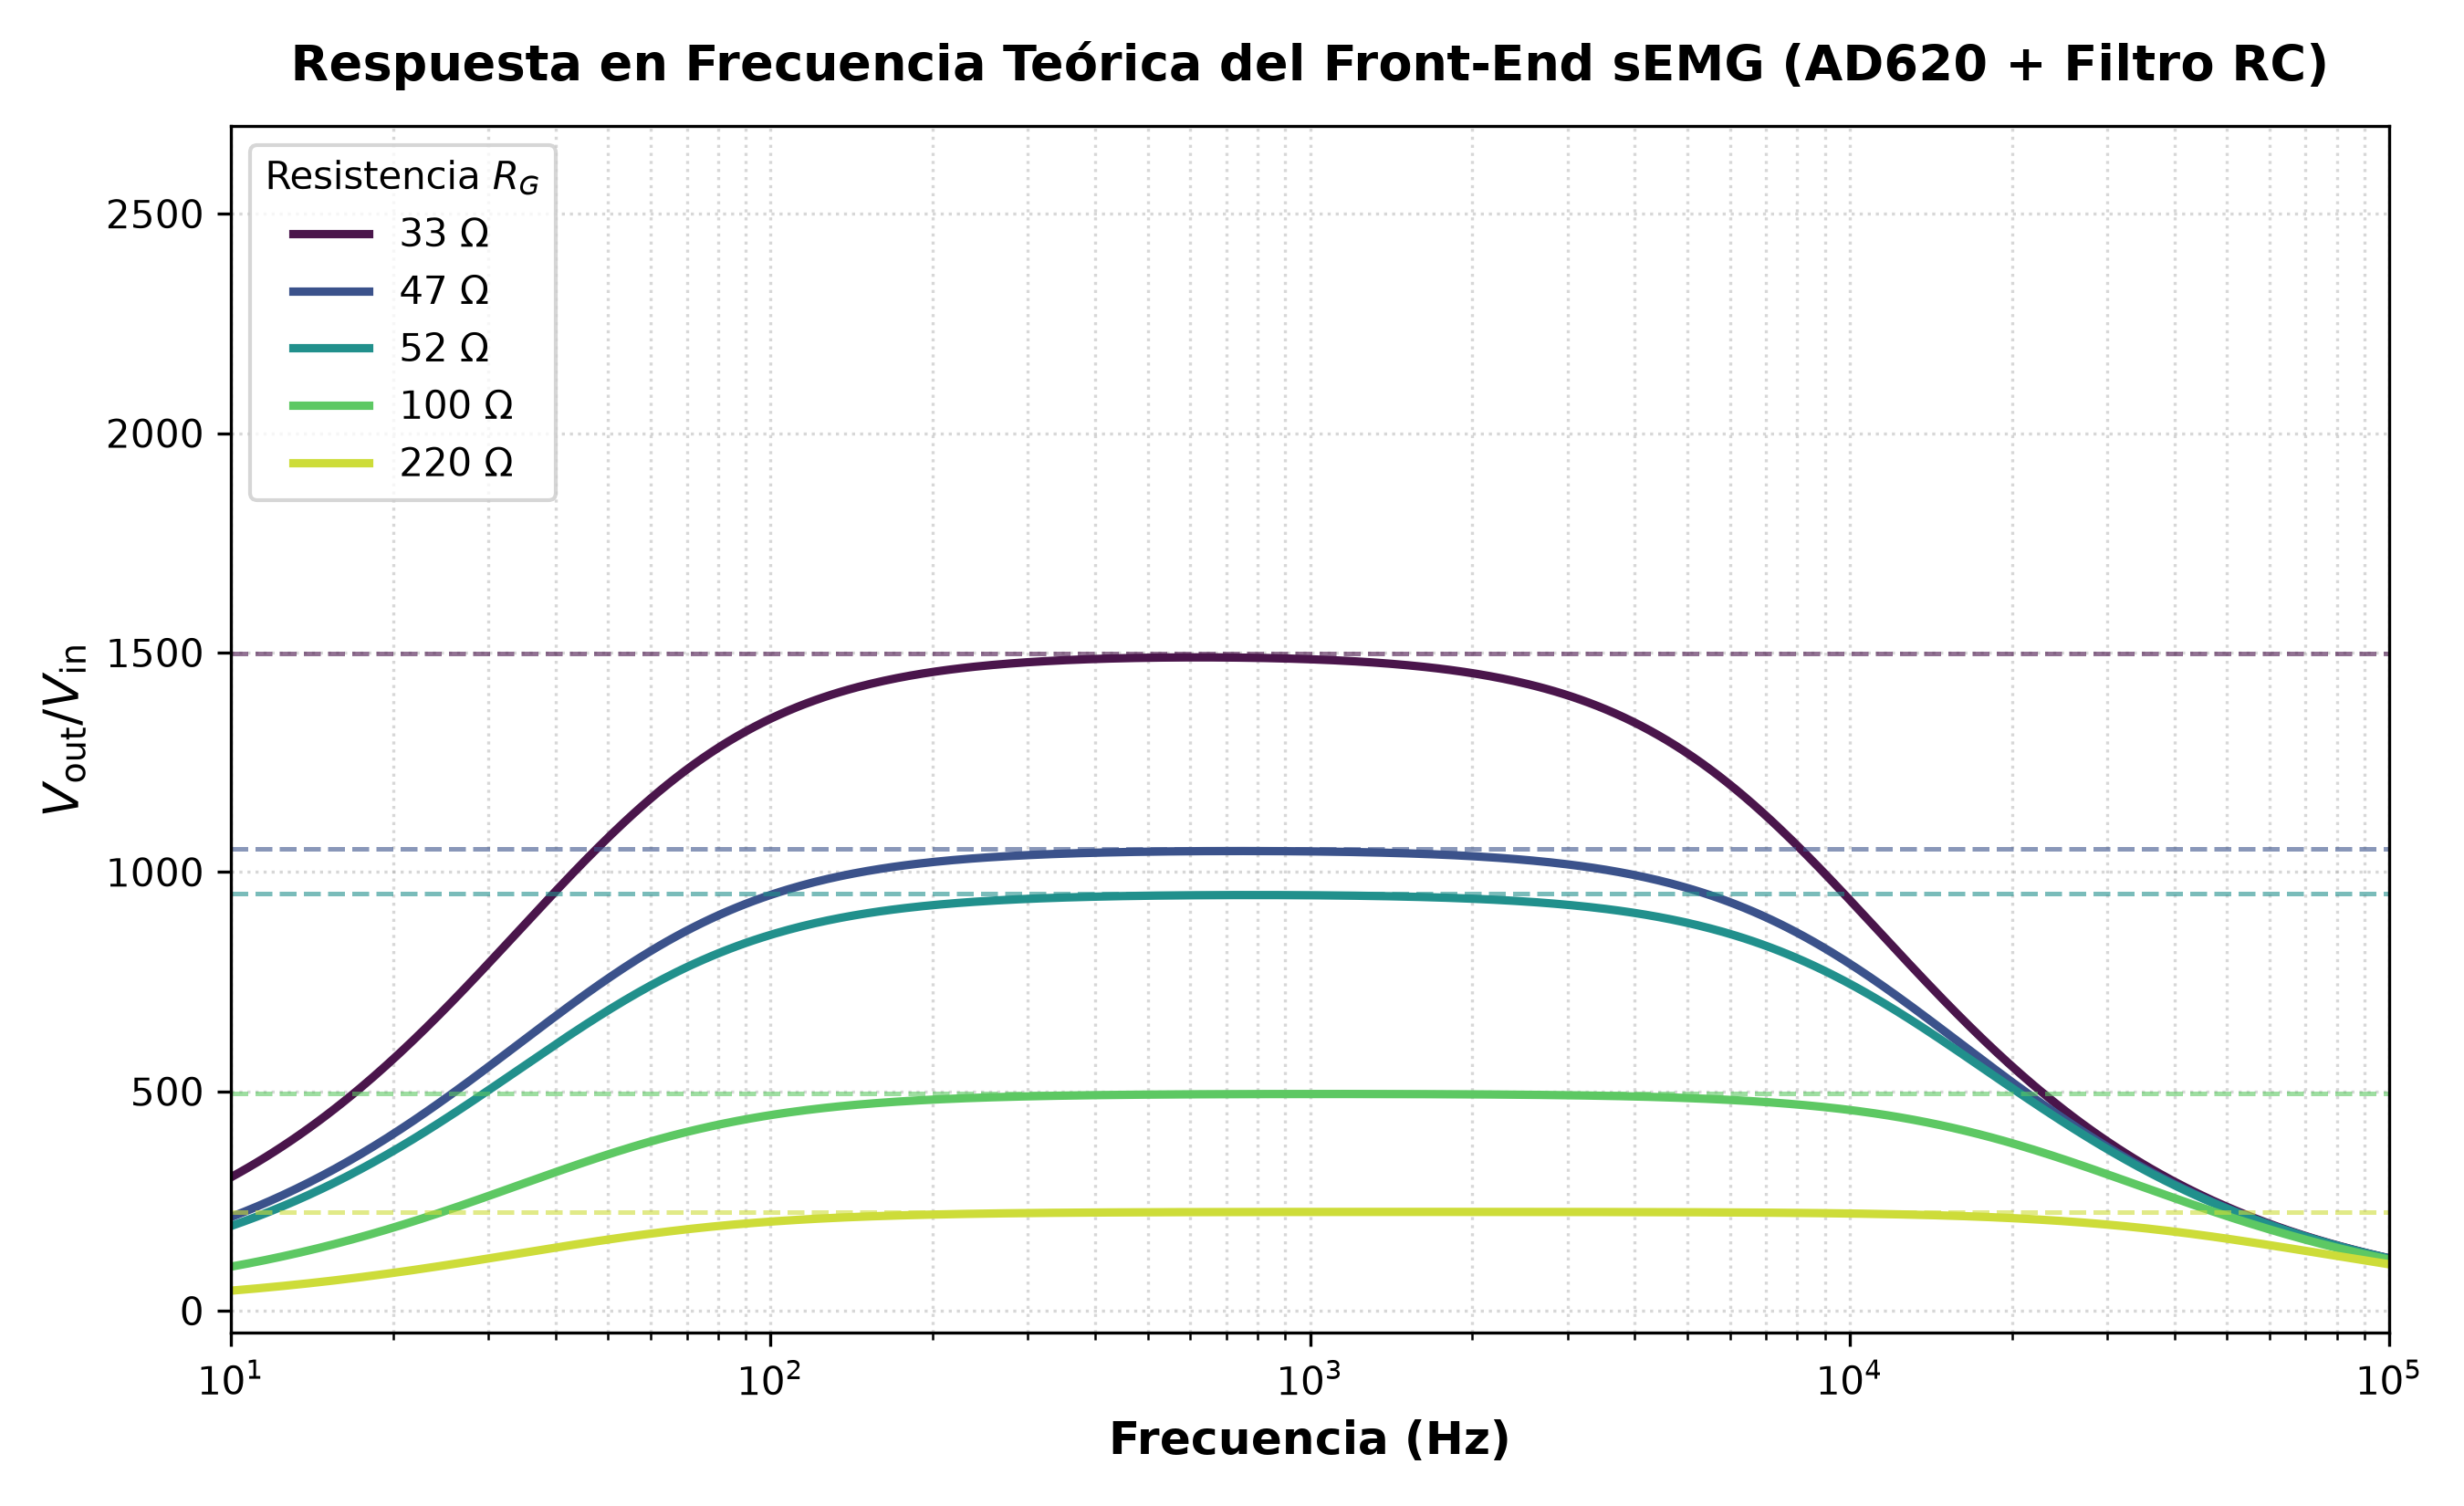
\includegraphics[width=\linewidth]{imagenes/curva_respuesta_frecuencia_teorica.png}
        \caption{Modelo analítico teórico}
        \label{fig:curva_teorica_inf}
    \end{subfigure}
    \caption{Curvas de amplificación en función de la resistencia $R_G$. Izquierda: mediciones experimentales en laboratorio con osciloscopio y generador. Derecha: respuesta en frecuencia teórica calculada según la función de transferencia del amplificador AD620 y la celda pasiva de entrada ($33\,\text{nF} + 100\,\text{k}\Omega$).}
    \label{fig:comparativa_frecuencia_inf}
\end{figure}

\subsection{Comparación entre el Circuito Actual y la Modificación de Impedancia}
Para subsanar el aplastamiento de impedancia ($Z_{\text{in}} \approx 100\,\text{k}\Omega$) y la pérdida de la banda sEMG orofacial por debajo de $48\,\text{Hz}$, la Figura \ref{fig:comparacion_resp_inf} compara la respuesta del hardware actual frente a la modificación propuesta (puenteo de capacitores de entrada, elevación de resistencias a $10\,\text{M}\Omega$ y capacitor $C_G = 100\,\mu\text{F}$ en serie con $R_G$).

\begin{figure}[H]
\centering
\resizebox{0.88\linewidth}{!}{%
\begin{circuitikz}[american, thick, font=\sffamily]

    % Marco delimitador con amplia holgura
    \draw[dashed, draw=green!60!black, fill=green!2, rounded corners] (-6.8, 4.4) rectangle (4.8, -3.8);
    \node[anchor=north west, font=\bfseries\color{green!50!black}] at (-6.5, 4.0) {CANAL CON MODIFICACI\'ON PROPUESTA: DESACOPLO AC EN LAZO DE GANANCIA};

    % AD620
    \draw[thick] (-0.6, 1.8) -- (2.6, 0) -- (-0.6, -1.8) -- cycle;
    \node at (0.9, 0) {\Large AD620};
    \node at (-0.2, 1.2) {\Large \(-\)};
    \node at (-0.2, -1.2) {\Large \(+\)};

    % Pines de Alimentación (±9V) y Referencia
    \draw[-latex] (0.4, 1.2) -- ++(0, 0.8) node[above, font=\small\bfseries\color{red!70!black}] {+9V};
    \node[left=1pt, font=\scriptsize] at (0.4, 1.4) {7};

    \draw[-latex] (0.4, -1.2) -- ++(0, -0.8) node[below, font=\small\bfseries\color{blue!70!black}] {-9V};
    \node[left=1pt, font=\scriptsize] at (0.4, -1.4) {4};

    \draw (1.4, -0.7) -- ++(0, -0.9) node[ground]{};
    \node[right=2pt, font=\scriptsize] at (1.4, -0.7) {5};

    \draw (2.6, 0) -- ++(1.4, 0) node[ocirc]{} node[pos=0.6, above, font=\scriptsize] {6} node[right, font=\small\bfseries] {$V_{\text{out}}$};

    % Lazo de ganancia horizontal (RG = 100 Ohm y CG = 100 uF para fc ≈ 16 Hz)
    \draw (-0.6, 0.5) node[right=2pt, font=\scriptsize] {1} 
          to[R, l_={\small $R_G = 100\,\Omega$}, *-*] (-2.6, 0.5) coordinate (rg_left);
    \draw (-0.6, -0.5) node[right=2pt, font=\scriptsize] {8} 
          to[C, l_={\small $C_G = 100\,\mu\text{F}$}, *-*] (-2.6, -0.5) coordinate (cg_left);
    \draw (rg_left) -- (cg_left);

    % Entradas directas acopladas en continua con alta impedancia (10 MOhm a GND)
    \draw (-0.6, 1.2) -- (-1.6, 1.2) -- (-1.6, 1.6) -- (-4.4, 1.6) coordinate (juncA);
    \draw (juncA) to[R, l_={\small $10\text{ M}\Omega$}] ++(0, 1.1) node[ground, yscale=-1]{};
    \draw (juncA) -- ++(-1.4, 0) node[left, font=\small\bfseries] {\(V_{\mathrm{in}}^-\)};

    \draw (-0.6, -1.2) -- (-1.6, -1.2) -- (-1.6, -1.6) -- (-4.4, -1.6) coordinate (juncB);
    \draw (juncB) to[R, l={\small $10\text{ M}\Omega$}] ++(0, -1.1) node[ground]{};
    \draw (juncB) -- ++(-1.4, 0) node[left, font=\small\bfseries] {\(V_{\mathrm{in}}^+\)};

\end{circuitikz}%
}
\caption{Esquema vectorial en \LaTeX{} (\texttt{circuitikz}) del canal sEMG con la modificación propuesta: entradas directas sin capacitores en serie, resistencias de polarización elevadas a $10\,\text{M}\Omega$ para maximizar la impedancia de entrada, y conexión en serie de $R_G = 100\,\Omega$ con el capacitor no polarizado $C_G = 100\,\mu\text{F}$ en el lazo de ganancia.}
\label{fig:circuito_modificado_vectorial_inf}
\end{figure}

\begin{figure}[htbp]
\centering
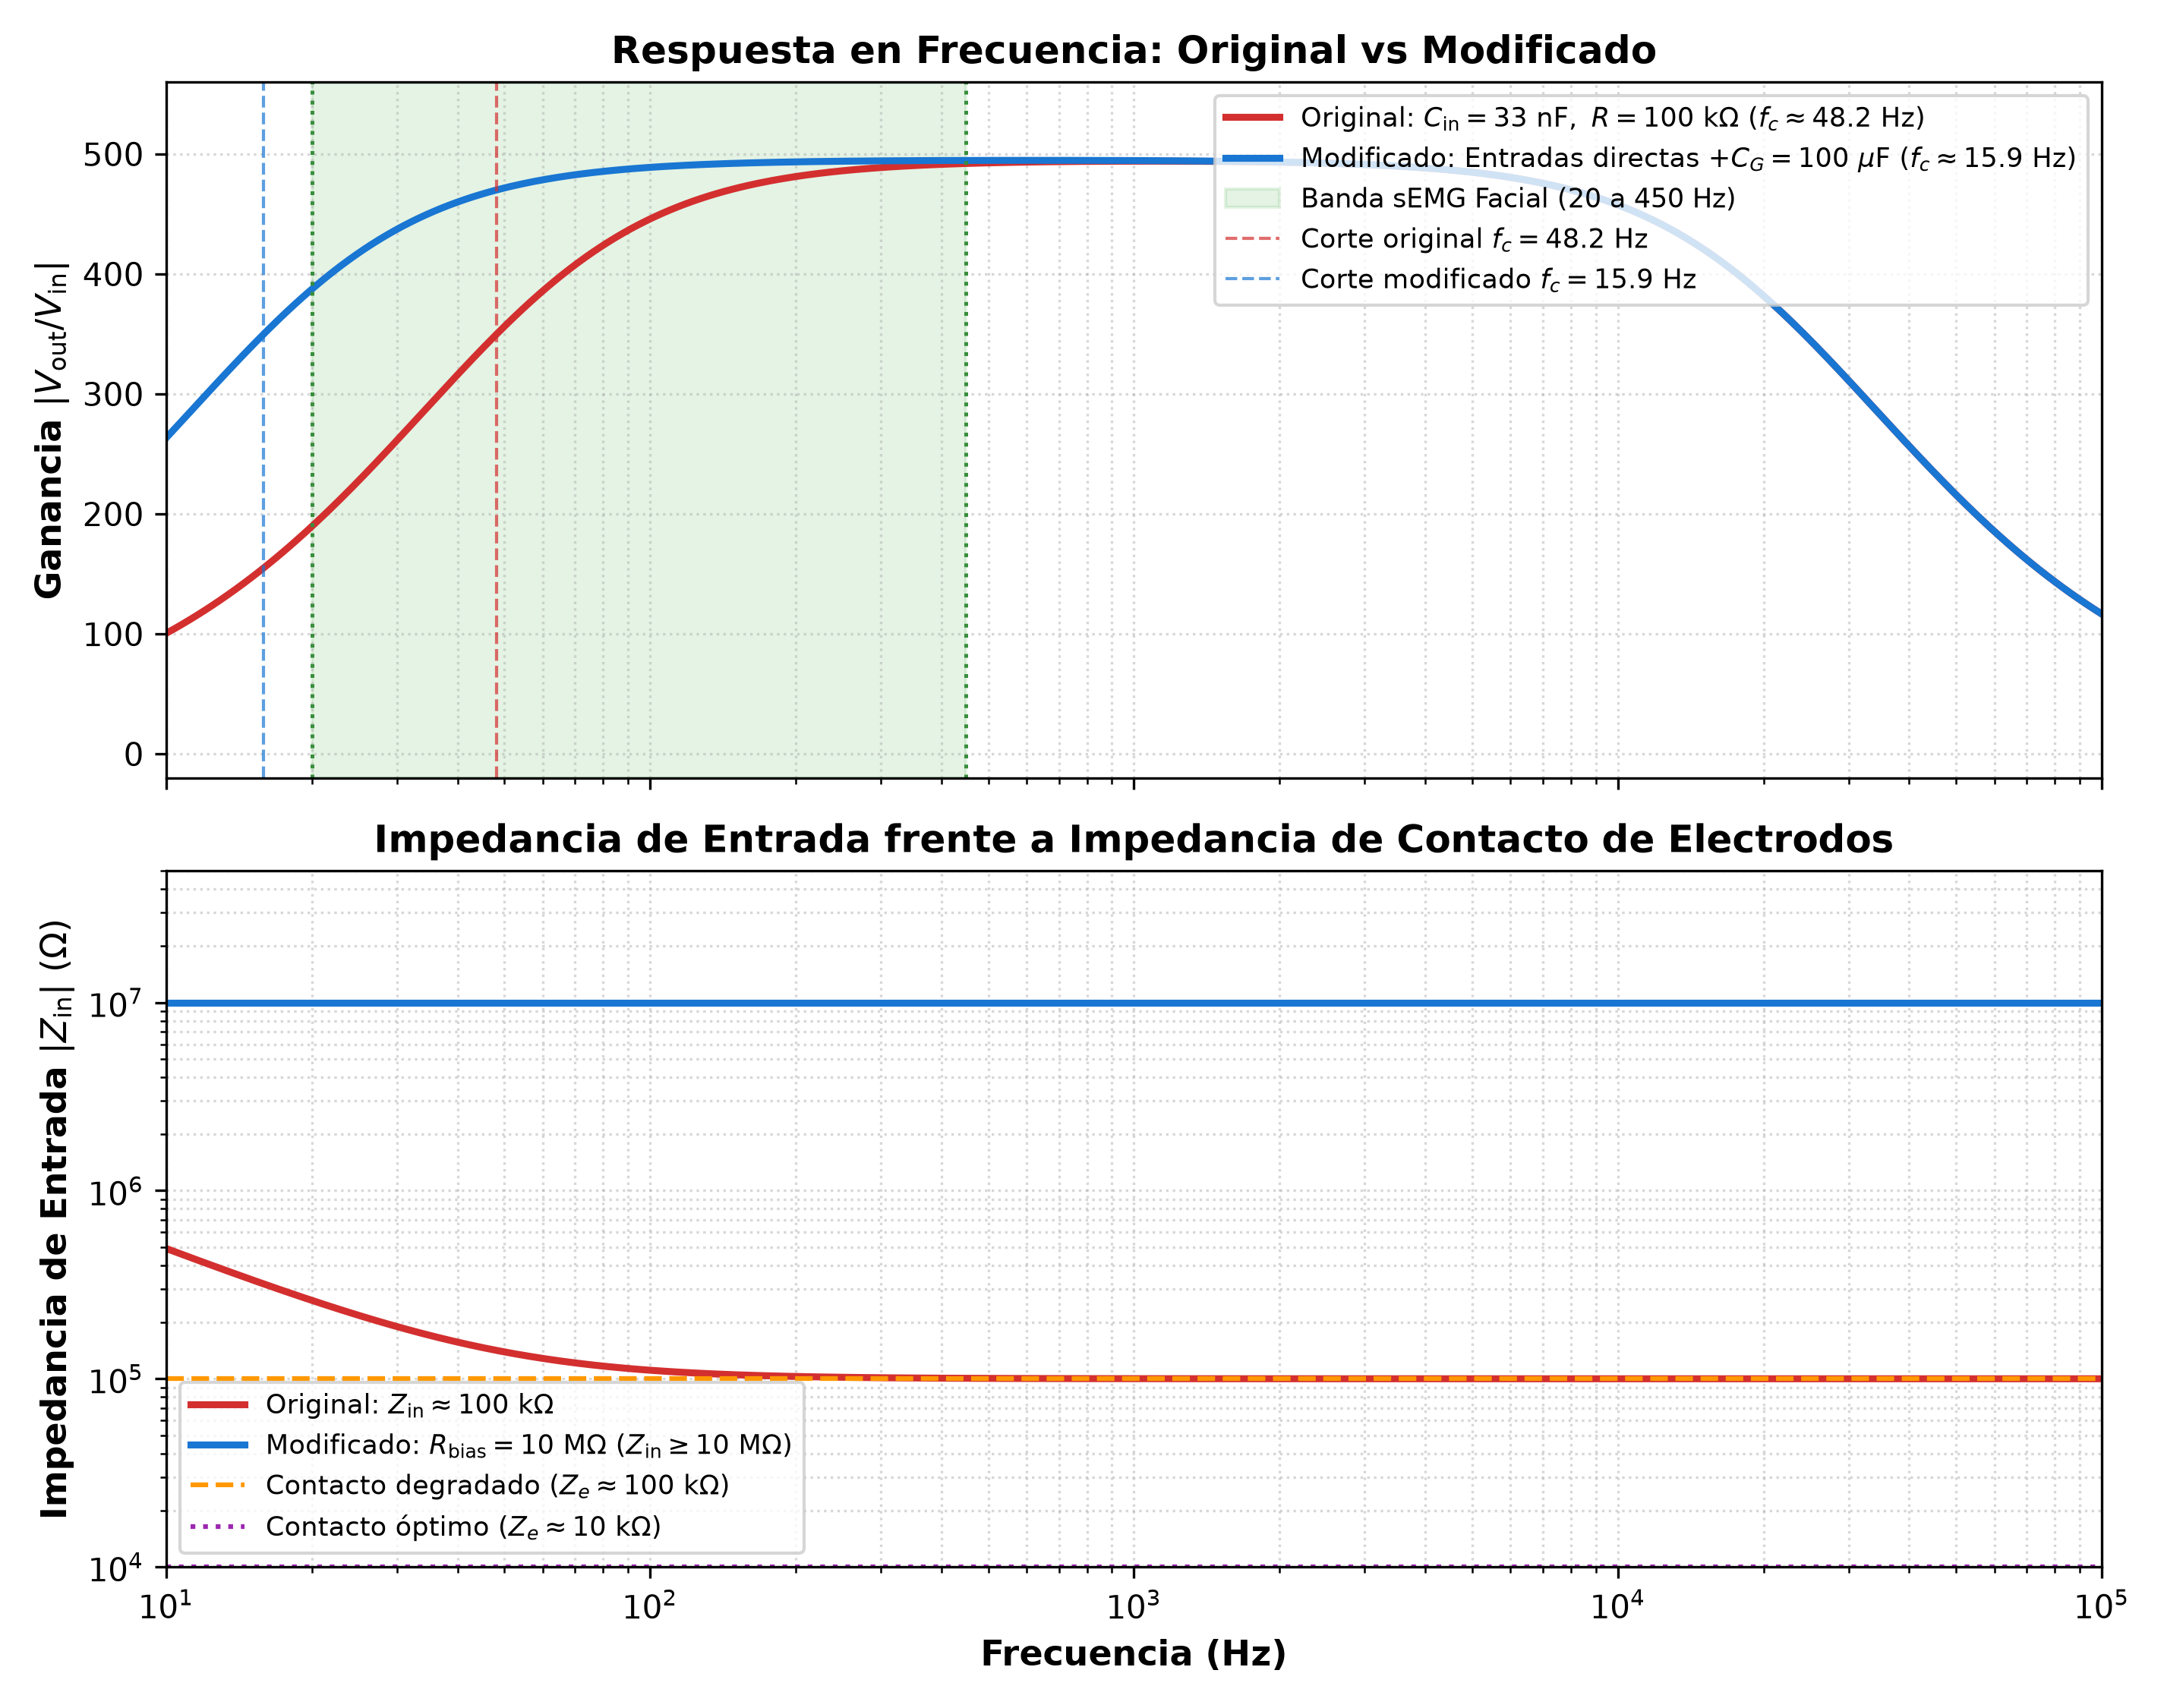
\includegraphics[width=0.88\textwidth]{imagenes/comparacion_respuesta_frecuencia_impedancia.png}
\caption{Comparación de desempeño entre el circuito original y la modificación de hardware propuesta. Superior: Ganancia en función de la frecuencia con recuperación de la banda sEMG facial (20 a 450 Hz) gracias al corte en $15.9\,\text{Hz}$. Inferior: Impedancia de entrada $Z_{\text{in}}$ frente a electrodos con degradación de contacto ($100\,\text{k}\Omega$).}
\label{fig:comparacion_resp_inf}
\end{figure}

\subsection{Lista Oficial de Materiales y Diseño Físico del PCB}
La Tabla \ref{tab:bom_inf} presenta la lista oficial y consolidada de materiales (BOM) para la fabricación del módulo sEMG.

\begin{table}[htbp]
\centering
\caption{Lista de materiales del módulo sEMG tricenal}
\label{tab:bom_inf}
\begin{tabular}{cllc}
\toprule
\textbf{Cant.} & \textbf{Componente} & \textbf{Descripción / Valor} & \textbf{Label} \\
\midrule
2 & Resistencia $10\,\text{k}\Omega$ & Película metálica $1/4\,\text{W}$, $\pm 1\%$ & $R_{1,3}$ \\
8 & Resistencia $100\,\text{k}\Omega$ & Película metálica $1/4\,\text{W}$, $\pm 1\%$ & $R_{1,2,5,4,7,8}$ y $R_{2,4}$ \\
3 & Resistencia $100\,\Omega$ & Película metálica $1/4\,\text{W}$, $\pm 1\%$ ($R_G$) & $R_{3,6,9}$ \\
6 & Capacitor $33\,\text{nF}$ & Cerámico multicapa $50\,\text{V}$ & $C_{1,2,3,4,5,6}$ \\
2 & Diodo Zener 1N4741A & Zener $11.0\,\text{V}$, $1.0\,\text{W}$ & $D_{1,2}$ \\
1 & MOSFET IRFZ44N & Canal N, $55\,\text{V}$, $49\,\text{A}$, TO-220 & $\text{MOS N}$ \\
1 & MOSFET F9540N & Canal P, $-100\,\text{V}$, $-19\,\text{A}$, TO-220 & $\text{MOS P}$ \\
3 & Amp. Op. AD620 & Amplificador de instrumentación, DIP-8 & $U_{1,2,3}$ \\
3 & Zócalo de 8 pines & Zócalo para circuito integrado DIP-8 & $U_{1,2,3}$ \\
2 & Portafusible & Portafusible para PCB $5 \times 20\,\text{mm}$ & $\text{FUSN/P}_{1,2}$ \\
2 & Fusible $0.25\,\text{A}$ & Fusible de vidrio de acción rápida & $\text{FUSE}_{1,2}$ \\
1 & Tira pines macho & Tira de pines rectos paso $2.54\,\text{mm}$ & -- \\
2 & Mini jumper & Jumper paso $2.54\,\text{mm}$ & -- \\
1 & Placa virgen epoxi & Placa de cobre virgen $15 \times 15\,\text{cm}$ & Sustrato \\
\bottomrule
\end{tabular}
\end{table}

El diseño de pistas, planos de masa y ubicación de borneras en la placa de circuito impreso se presenta en la Figura \ref{fig:layout_pcb_inf}.

\begin{figure}[htbp]
\centering
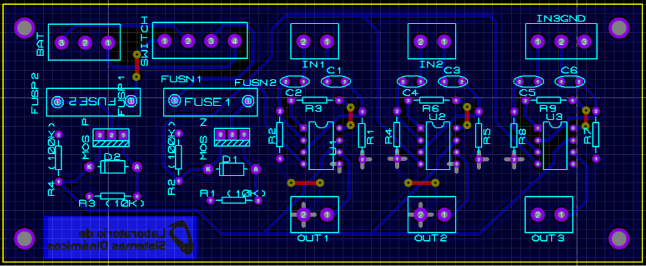
\includegraphics[width=0.88\textwidth]{imagenes/layout_pcb_completo.png}
\caption{Diseño del circuito impreso (PCB Layout) con serigrafía del Laboratorio de Sistemas Dinámicos.}
\label{fig:layout_pcb_inf}
\end{figure}

% ====================================================================
\section{Conclusiones}
% ====================================================================
\begin{enumerate}
    \item La colocación de capacitores en las entradas de un amplificador de instrumentación degrada el CMRR debido a tolerancias físicas y aplasta la impedancia de entrada, convirtiendo los $50\,\text{Hz}$ en ruido diferencial ante cualquier despegue.
    \item La modificación mediante desacoplo AC en $R_G$ ($100\,\Omega + 100\,\mu\text{F}$) junto con resistencias de $10\,\text{M}\Omega$ a GND resuelve la saturación DC y mitiga el ruido sin necesidad de fabricar un nuevo PCB.
    \item La arquitectura de dos etapas recomendada por SENIAM (AD620 a $G \approx 10$ + TL072 a $G = 48$ con corte a $500\,\text{Hz}$) constituye la solución óptima y definitiva para la versión final del sistema de adquisición.
\end{enumerate}

\end{document}
